% Created 2017-03-20 Mon 10:20
% Intended LaTeX compiler: pdflatex
\documentclass[10pt,aspectratio=1610]{beamer}
\usepackage[utf8]{inputenc}
\usepackage[T1]{fontenc}
\usepackage{graphicx}
\usepackage{grffile}
\usepackage{longtable}
\usepackage{wrapfig}
\usepackage{rotating}
\usepackage[normalem]{ulem}
\usepackage{amsmath}
\usepackage{textcomp}
\usepackage{amssymb}
\usepackage{capt-of}
\usepackage{hyperref}
\usepackage[english]{babel}\usepackage{etex}\usepackage{minted}\usemintedstyle{emacs}
\usepackage{tikz}\usepackage{amsmath}\usepackage[T1]{fontenc}\usepackage{lmodern}%\usepackage{arev}
\usepackage{booktabs}\usepackage[citestyle=alphabetic,bibstyle=authortitle]{biblatex}
\usepackage{pgfplots,pgfplotstable}\usetikzlibrary{pgfplots.groupplots}\usepackage[babel=true,kerning=true]{microtype}\usepackage{smartdiagram}
\addbibresource{fe.bib}
\usetikzlibrary{mindmap,trees,shapes,arrows,spy,3d,decorations.pathmorphing,pgfplots.statistics,pgfplots.dateplot}
\pgfplotsset{compat=newest}
\usetheme{DarkConsole}
\author{Mathieu Fauvel}
\date{\textit{[2017-04-26 Wed 10:30]--[2017-04-26 Wed 12:00]}}
\title{Feature Extraction}
\subtitle{GRSS Summer School}
\institute{UMR Dynafor}
\AtBeginSection[]{\begin{frame}<beamer>\frametitle{Outline}\tableofcontents[currentsection]\end{frame}}
\AtBeginSubsection[]{\begin{frame}<beamer>\frametitle{Outline}\tableofcontents[currentsubsection]\end{frame}}
\setbeamercovered{again covered={\opaqueness<1->{25}}}
\usefonttheme[onlymath]{serif}
\begin{document}

\maketitle
\begin{frame}{Outline}
\tableofcontents
\end{frame}

\section{Motivations}
\label{sec:org98dfc9c}
\begin{frame}[label={sec:org0d3d101}]{Illustration}
\begin{itemize}
\item <1-> \alert{Curse of dimensionality}: it is not possible to get enough data to cover all the observation space.
\begin{center}
\emph{High dimensional saces are mostly empty !}
\end{center}
\item <2> Multivariate data live in a lower dimensional space
\begin{center}
  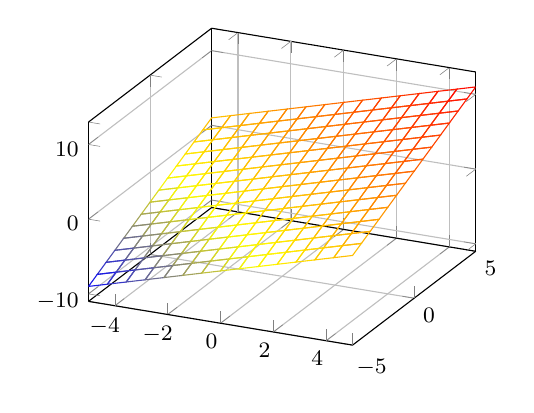
\begin{tikzpicture}
    \begin{axis}[grid=major,small]
      \addplot3 [mesh, samples=15, domain=-5:5] {x+y+1};
    \end{axis}
  \end{tikzpicture}
\end{center}
\end{itemize}
\end{frame}
\begin{frame}[label={sec:orgfde4e1e}]{Application}
\begin{itemize}
\item Feature extraction is important in remote sensing because:
\begin{itemize}
\item It reduces the size of the data,
\item It limits the spatial and spectral redundancy,
\item It permits visualization of the data,
\item It mitigates the \emph{curse of dimensionality}.
\end{itemize}
\item Extraction techniques:
\begin{itemize}
\item Spectral
\begin{itemize}
\item Physically based method,
\item Statistical methods.
\end{itemize}
\item Spatial:
\begin{itemize}
\item Linear filters,
\item Non linear techniques (Mathematical Morphology)
\end{itemize}
\end{itemize}
\end{itemize}
\end{frame}

\section{Physical Indices}
\label{sec:org0d81d32}
\subsection{Introduction}
\label{sec:org25e504a}
\begin{frame}[label={sec:org0d91760}]{Spectral indices}
\begin{itemize}
\item Spectral indices are a linear/non-linear combination of two (or more) spectral bands.
\item They provides information as a \emph{single number} about:
\begin{itemize}
\item Plant structure,
\item Biochemistry,
\item Humidity,
\item Stress.
\end{itemize}
\item Four main types \cite{hrsv:2011}:
\begin{center}
\begin{tabular}{ll}
\toprule
Name & Formulae\\
\midrule
Difference vegetation index & \(R_{\lambda_1} - R_{\lambda_2}\)\\
Ratio vegetation index & \(\dfrac{R_{\lambda_1}}{R_{\lambda_2}}\)\\
Normalized difference vegetation index & \(\dfrac{R_{\lambda_1} - R_{\lambda_2}}{R_{\lambda_1} + R_{\lambda_2}}\)\\
Soil-adjusted vegetation index & \((1+L)\times\dfrac{R_{\lambda_1} - R_{\lambda_2}}{R_{\lambda_1} - R_{\lambda_2}+L}\)\\
\bottomrule
\end{tabular}
\end{center}
\item \emph{The three last indexes are invariant to  a multiplicative factor}
\end{itemize}
\end{frame}

\begin{frame}[label={sec:orgefa99f0}]{Conventional Indices}
Index database : \url{http://www.indexdatabase.de/}

\begin{center}
\small
\begin{tabular}{ll}
\toprule
Name & Formulae  (\(\lambda\) nm)\\
\midrule
Normalized Difference Vnegetation index & \(\dfrac{R_{\lambda_{800}} - R_{\lambda_{670}}}{R_{\lambda_{800}} + R_{\lambda_{670}}}\)\\
Modified Soil-Adjusted Vegetation Index & \(\dfrac{1}{2}\left[2R_{\lambda_{800}}+1 - \sqrt{(2R_{\lambda_{800}}+1)^2-8(R_{\lambda_{800}}-R_{\lambda_{670}})}\right]\)\\
Modified Chlorophyll Absorption Ratio Index & \(\left[(R_{\lambda_{700}}-R_{\lambda_{670}})-0.2(R_{\lambda_{700}}-R_{\lambda_{550}})\right]\times\dfrac{R_{\lambda_{700}}}{R_{\lambda_{670}}}\)\\
\midrule
Normalized Difference Water Index & \(\dfrac{R_{\lambda_{858}} - R_{\lambda_{1240}}}{R_{\lambda_{858}} + R_{\lambda_{1240}}}\)\\
Datt Reflectance Index & \(\dfrac{R_{\lambda_{816}} - R_{\lambda_{2218}}}{R_{\lambda_{816}} + R_{\lambda_{2218}}}\)\\
\midrule
Normalized Difference Redness Index & \(\dfrac{R_{\lambda_{540}} - R_{\lambda_{700}}}{R_{\lambda_{540}} + R_{\lambda_{700}}}\)\\
Soil Brightness Index & \(0.406R_{\lambda{550}}+0.600R_{\lambda{650}}+0.645R_{\lambda{750}}+0.243R_{\lambda{950}}\)\\
\bottomrule
\end{tabular}
\end{center}
\end{frame}

\subsection{Vegetation Indices}
\label{sec:org069bf83}
\begin{frame}[label={sec:orgc8b3ae1}]{Normalized difference vegetation index}
$$\text{NDVI}=\dfrac{R_{\lambda_{800}} - R_{\lambda_{670}}}{R_{\lambda_{800}} + R_{\lambda_{670}}}$$
\begin{itemize}
\item \(-1\leq \text{NVDI} \leq 1\)
\item \(\text{NDVI}< 0\): surfaces other thatn plant cover
\item \(\text{NDVI}\approx 0\): bare soil
\item \(\text{NDVI}\geq 0.1\): vegetation cover (higher values correspond to more dense covers)
\end{itemize}

\begin{center}
\begin{tikzpicture}
\begin{axis}[xmin=0.4,xmax=1,ymin=0,ymax=1,grid,xlabel=$\lambda~({\mu}m)$,ylabel=Reflectance,width=0.6\linewidth,height=0.3\linewidth,cycle list name=color list]
  \addplot+[mark=none,thick,smooth] file {../Introduction/figures/oak.txt};
  \pgfplotstableread{../Introduction/figures/grass.txt}\loadedtable
  \addplot+[mark=none,smooth,thick] table[x=wave,y=grass] from \loadedtable;
  \addplot+[mark=none,smooth,thick] table[x=wave,y=drygrass] from \loadedtable;
  \pgfplotstableread{../Introduction/figures/talc.txt}\loadtable
  \addplot+[mark=none,smooth,thick] table[x=wave,y=talc] from \loadtable;
  \legend{0.81,0.90, 0.05, -0.03}
\end{axis}
\end{tikzpicture}
\end{center}
\end{frame}
\subsection{Case study}
\label{sec:org5f62678}
\begin{frame}[label={sec:orga174e52}]{University of Pavia}
\begin{columns}
\begin{column}{0.5\columnwidth}
\begin{center}
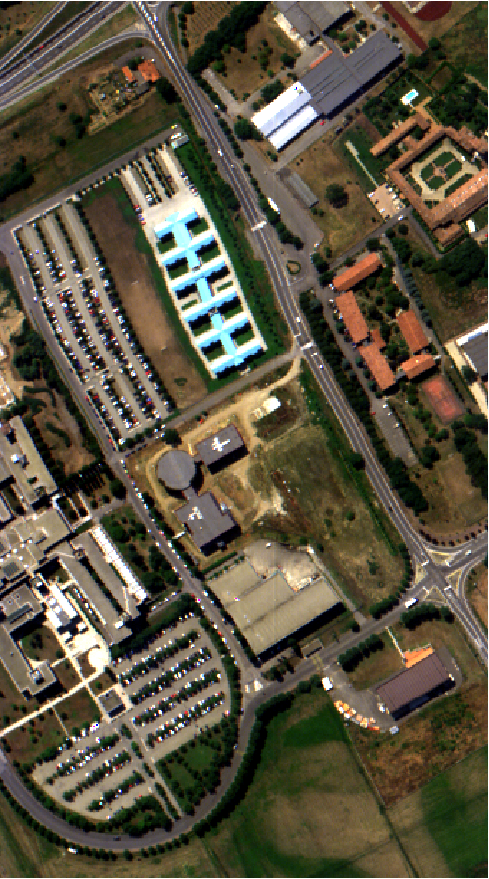
\includegraphics[width=0.6\linewidth]{./figures/university_color.png}
\end{center}
\end{column}

\begin{column}{0.5\columnwidth}
\begin{itemize}
\item Peri-urban area
\item Rosis-3 sensor
\item 103 Spectral bands (400nm-900nm)
\item 1.5 meter per pixel spatial resolution
\item 610 \(\times\) 340 pixels
\end{itemize}
\end{column}
\end{columns}
\end{frame}

\begin{frame}[fragile,label={sec:org4605749}]{Orfeo-Toolbox}
 \begin{itemize}
\item \href{https://www.orfeo-toolbox.org/}{OTB} is a C++ library for remote sensing images processing.
\item It is free, open-source and available for most OS (window, apple, linux)
\item \href{https://www.orfeo-toolbox.org/CookBook/OTB-Applications.html}{OTB-Applications} are set of tools appropriated for big/large images
\item They are avalaible from QGIS, Python and Bash
\item To compute the NDVI
\end{itemize}

\begin{minted}[fontsize=\footnotesize,obeytabs=true,tabsize=4,bgcolor=bg]{bash}
# Computation of the NDVI
otbcli_BandMath -il ../Data/university.tif -out ../Data/university_ndvi.tif \
		-exp "(im1b83-im1b56)/(im1b83+im1b56)"

# Computation of the SBI
otbcli_BandMath -il ../Data/university.tif -out ../Data/university_sbi.tif \
		-exp "0.406*im1b31 + 0.6*im1b52 + 0.645*im1b73"
\end{minted}
\end{frame}

\begin{frame}[label={sec:org0d26203}]{University of Pavia - Spectral Indices}
\begin{columns}
\begin{column}{0.3\columnwidth}
\begin{center}
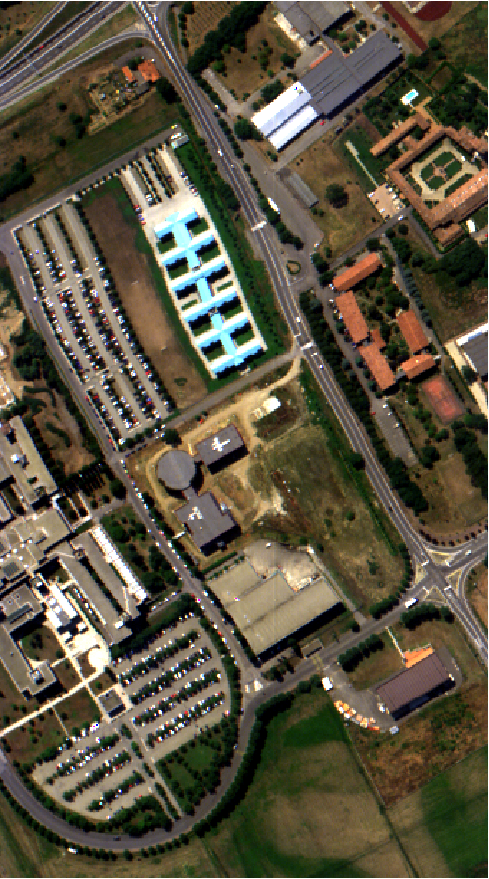
\includegraphics[width=\linewidth]{./figures/university_color.png}
\end{center}
\end{column}

\begin{column}{0.3\columnwidth}
\begin{center}
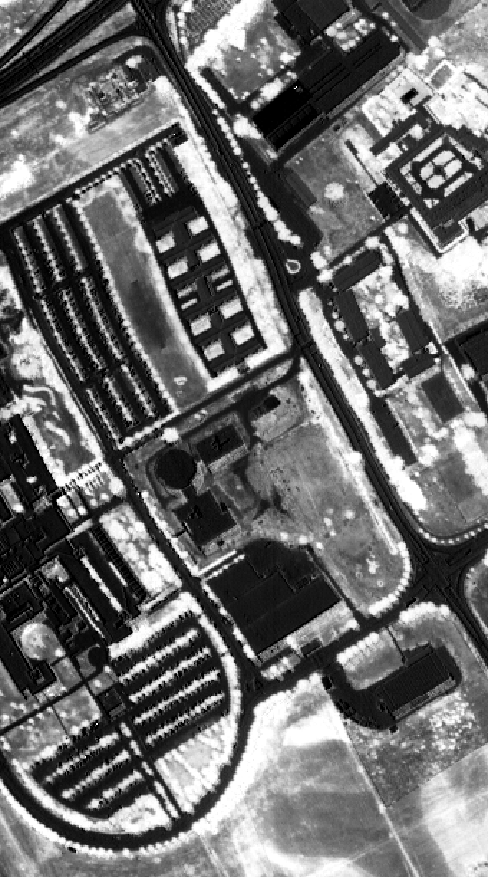
\includegraphics[width=\linewidth]{./figures/university_ndvi.png}
\end{center}
\end{column}

\begin{column}{0.3\columnwidth}
\begin{center}
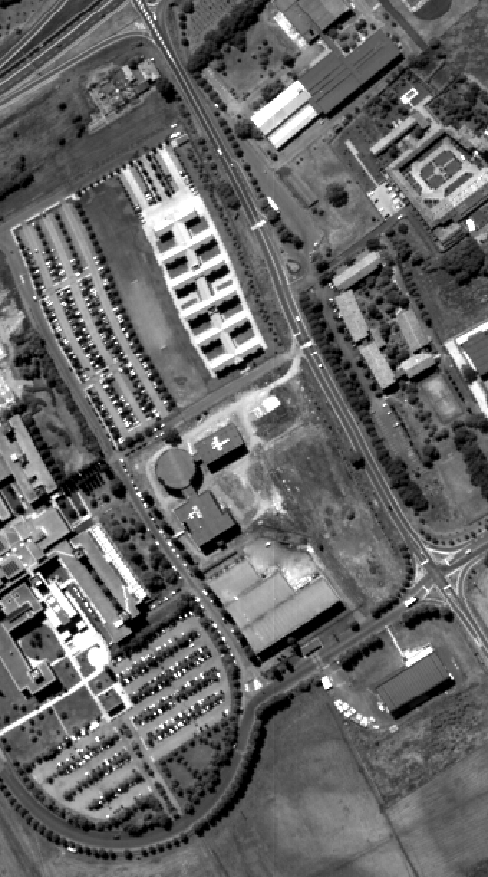
\includegraphics[width=\linewidth]{./figures/university_sbi.png}
\end{center}
\end{column}
\end{columns}
\end{frame}

\begin{frame}[fragile,label={sec:org140ce2e}]{Where is the vegetation 1/2 ?}
   \begin{center}
  \begin{tikzpicture}
    \begin{axis}[grid=both,width=0.95\linewidth,height=0.45\linewidth,/pgf/number format/1000 sep={},/pgf/number format/fixed,title=Density plot of the NDVI,xmin=-0.6,xmax=1,ymin=0,ymax=0.01]
      \addplot+[mark=none,thick,smooth] table[x=x,y=y,col sep=comma] {figures/pdf.csv};
      \only<2->{\addplot[red,thick] coordinates {(0.19,0) (0.19,0.008)};
      \addplot[red,thick] coordinates {(0.62,0) (0.62,0.008)}; }     
    \end{axis}
\end{tikzpicture}
\end{center}

\begin{minted}[fontsize=\footnotesize,obeytabs=true,tabsize=4,bgcolor=bg]{bash}
# Segmentation of the NDVI in three classes
otbcli_BandMath -il ../Data/university_ndvi.tif -out ../Data/university_ndvi_segmented.tif \
		-exp "(im1b1<0.19?1:(im1b1<0.62?2:3))"
\end{minted}
\end{frame}

\begin{frame}[label={sec:org441526a}]{Where is the vegetation 2/2 ?}
\begin{columns}
\begin{column}{0.5\columnwidth}
\begin{center}
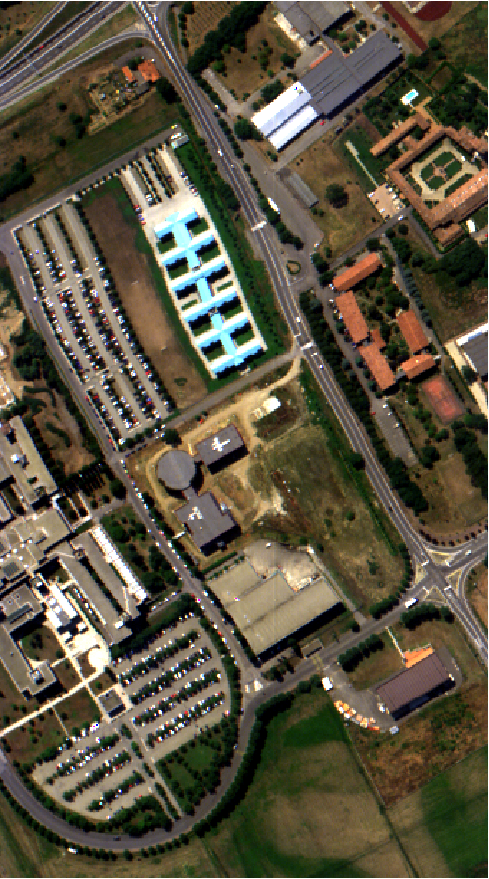
\includegraphics[width=0.6\linewidth]{./figures/university_color.png}
\end{center}
\end{column}

\begin{column}{0.5\columnwidth}
\begin{center}
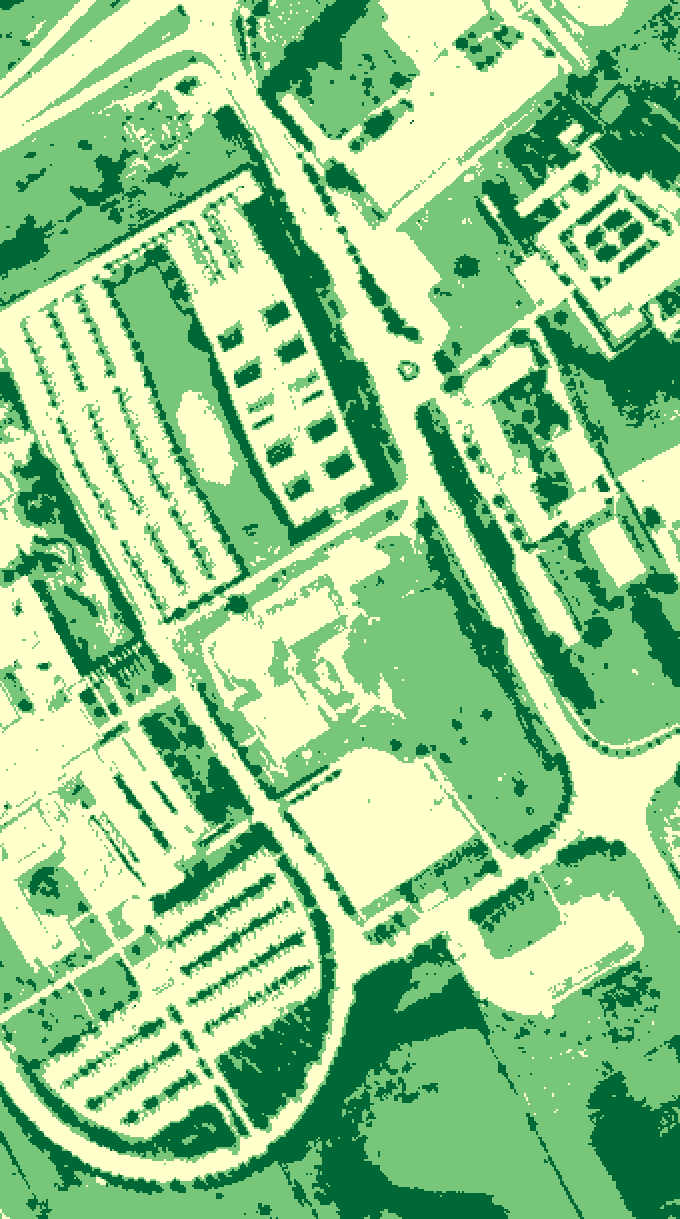
\includegraphics[width=0.6\linewidth]{./figures/university_ndvi_segmented.png}
\end{center}
\end{column}
\end{columns}
\end{frame}

\subsection{Question}
\label{sec:org9a31650}
\begin{frame}[label={sec:org2fe6abd}]{Could you find the good one ?}
 \centerline{\begin{tabular}{cc}
    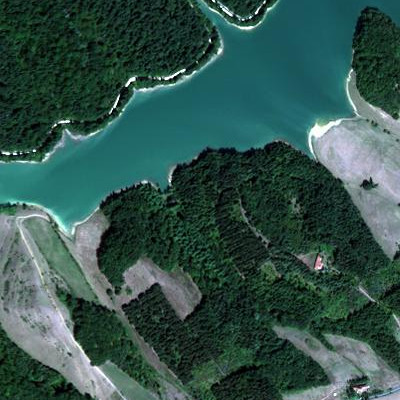
\includegraphics[width=0.4\linewidth]{figures/image1.jpg} & \begin{tikzpicture}\pgfplotsset{every axis legend/.append style={at={(0.5,1.03)},anchor=south}}
      \begin{axis}[ytick=\empty,xmin=-0.5,xmax=0.9,ymin=0,width=0.5\linewidth,axis y line=center,axis x line=bottom,legend columns=4]
        \pgfplotstableread{figures/ndvi1.txt}\loadedtable
        \addplot[smooth,very thick,dashed,blue] table[x=wave,y=ndvi] from \loadedtable;
        \pgfplotstableread{figures/ndvi2.txt}\loadedtable
        \addplot[smooth,very thick,magenta] table[x=wave,y=ndvi] from \loadedtable;
        \pgfplotstableread{figures/ndvi3.txt}\loadedtable
        \addplot[smooth,very thick,dotted,orange] table[x=wave,y=ndvi] from \loadedtable;
        \pgfplotstableread{figures/ndvi4.txt}\loadedtable
        \addplot[smooth,very thick,dashdotted,green] table[x=wave,y=ndvi] from \loadedtable;
        \legend{ndvi$_1$,ndvi$_2$,ndvi$_3$,ndvi$_4$};
      \end{axis}
    \end{tikzpicture}\\
    Image & NDVI Histogram
\end{tabular}}
\vspace{1cm}

From the histogram, which one does correspond to the NDVI of the image ?
\end{frame}
\section{Statistical Feature Extraction}
\label{sec:org241aefd}
\subsection{Unsupervised}
\label{sec:org18e55d5}
\begin{frame}[label={sec:orgddeea9f}]{Principal Components Analysis}
\begin{itemize}
\item Linear transformation used to reduce the dimensionality of the data \cite{jolliffe2002principal}.
$$ z_i = \langle\mathbf{v}_i,\mathbf{x}\rangle$$
\item Find features \(\mathbf{z}\) that  account for most of the variability of the data:
\begin{itemize}
\item \(z_1,~z_2,~z_3,\ldots\) are mutually uncorrelated,
\item \(\text{var}(z_i)\) is as large as possible,
\item \(\text{var}(z_1)>\text{var}(z_2)>\text{var}(z_3)>\ldots\)
\end{itemize}
\end{itemize}

\begin{center}
  \begin{tikzpicture}
    \begin{axis}[grid,small,width=0.4\linewidth,height=0.32\linewidth,xmin=0,xmax=2.5,ymin=0,ymax=2]
      \addplot[only marks,blue] table[x index=0,y index = 1,col sep =comma] {figures/pca_data.csv};
      \begin{scope}
      \addplot[very thick,red] coordinates { (0.080264,0.83834891)  (2.06023219,1.12070676)};
      \addplot[very thick,red] coordinates { (0.92906917,  1.96951193)(1.21142702, -0.01045626)};
    \end{scope}

   \end{axis}                                  
  \end{tikzpicture}
\end{center}
\end{frame}
\begin{frame}[label={sec:org15e9748}]{Maximization of the variance 1/2}
\begin{itemize}
\item <1-> Search \(\mathbf{v}_1\) such as \(\max\text{var}(z_1)\):
\begin{eqnarray*}
  \text{var}(z_1) & = & \text{var}(\langle\mathbf{v}_1,\mathbf{x}\rangle)\\
  &=& \mathbf{v}_1^\top\boldsymbol{\Sigma}\mathbf{v}_1
\end{eqnarray*}
\item <2-> Indetermined: if \(\hat{\mathbf{v}}_1\) maximizes the variance, \(\alpha\hat{\mathbf{v}}_1\) too!  Add a constraint: \(\langle\mathbf{v}_1,\mathbf{v}_1\rangle=1\)
\item <3-> Lagrangian:
\begin{eqnarray*}
  \mathcal{L}(\mathbf{v}_1,\lambda_1) = \mathbf{v}_1^\top\boldsymbol{\Sigma}\mathbf{v}_1 + \lambda_1(1- \mathbf{v}_1^\top\mathbf{v}_1)  
\end{eqnarray*}
\item <4-> Compute the derivative w.r.t \(\mathbf{v}_1\):
\begin{eqnarray*}
\frac{\partial\mathcal{L}}{\partial\mathbf{v}_1} = 2\boldsymbol{\Sigma}\mathbf{v}_1-2\lambda_1\mathbf{v}_1
\end{eqnarray*}
\item <5-> \(\mathbf{v}_1\) is an eigenvector of the covariance matrix of \(\mathbf{x}\):
\begin{eqnarray*}
  \boldsymbol{\Sigma}\mathbf{v}_1 =\lambda_1\mathbf{v}_1
\end{eqnarray*}
\item <6->  \(\mathbf{v}_1\) is the eigenvector corresponding to the largest eigenvalues !
\begin{eqnarray*}
  \text{var}(z_1)  =  \mathbf{v}_1^\top\boldsymbol{\Sigma}\mathbf{v}_1 = \lambda_1 \mathbf{v}_1^\top\mathbf{v}_1 = \lambda_1
\end{eqnarray*}
\end{itemize}
\end{frame}
\begin{frame}[label={sec:org988812e}]{Maximization of the variance 2/2}
\begin{itemize}
\item <1-> Search \(\mathbf{v}_2\) such as \(\max\text{var}(z_2)\) and \(\langle\mathbf{v}_2,\mathbf{v}_2\rangle=1\) and \(\langle\mathbf{v}_1,\mathbf{v}_2\rangle=0\)
\item <2-> Lagrangian:
\begin{eqnarray*}
  \mathcal{L}(\mathbf{v}_2,\lambda_2,\beta_1) = \mathbf{v}_2^\top\boldsymbol{\Sigma}\mathbf{v}_2 + \lambda_1(1- \mathbf{v}_2^\top\mathbf{v}_2) + \beta_1(0 - \mathbf{v}_2^\top\mathbf{v}_1)
\end{eqnarray*}
\item <3-> Compute the derivative w.r.t \(\mathbf{v}_2\):
\begin{eqnarray*}
\frac{\partial\mathcal{L}}{\partial\mathbf{v}_2} &=& 2\boldsymbol{\Sigma}\mathbf{v}_2-2\lambda_1\mathbf{v}_2-\beta_1\mathbf{v}_1\\
\boldsymbol{\Sigma}\mathbf{v}_2 &=& \lambda_1\mathbf{v}_2+2\beta_1\mathbf{v}_1
\end{eqnarray*}
\item <4-> At optimality, \(\langle\mathbf{v}_1,\mathbf{v}_2\rangle=0\). Left-multiplying by \(\mathbf{v}_1^\top\) the above equation:
\begin{eqnarray*}
  \mathbf{v}_1^\top\boldsymbol{\Sigma}\mathbf{v}_2 &=& 2\beta_1 \\
  \lambda_1\mathbf{v}_1^\top\mathbf{v}_2 &=& 2\beta_1 \\
  0 &=& 2\beta_1 \\
\end{eqnarray*}
\item <5-> Hence, we have 
\begin{eqnarray*}
  \boldsymbol{\Sigma}\mathbf{v}_2 =\lambda_2\mathbf{v}_2
\end{eqnarray*}
\item <6-> \(\mathbf{v}_2\) is the eigenvector corresponding the \emph{second largest} eigenvalues
\item <7-> \(\mathbf{v}_k\) is the eigenvector corresponding the \emph{\(k^{\text{th}}\) largest} eigenvalues
\end{itemize}
\end{frame}
\begin{frame}[label={sec:orgeadec90}]{PCA in practice}
\begin{enumerate}
\item Empirical estimation the mean value:
\begin{eqnarray*}
  \boldsymbol{\mu} = \frac{1}{n}\sum_{i=1}^n\mathbf{x}_i
\end{eqnarray*}
\item Empirical estimation the covariance matrix:
\begin{eqnarray*}
  \boldsymbol{\Sigma} = \frac{1}{n-1}\sum_{i=1}^n(\mathbf{x}_i-\boldsymbol{\mu})(\mathbf{x}_i-\boldsymbol{\mu})^\top
\end{eqnarray*}
\item Compute \(p\) first eigenvalues/eigenvectors\ldots{} How to choose \(p\) ? Explained variance: 
$$\frac{\sum_{i=1}^p\lambda_i}{\sum_{i=1}^d\lambda_i}$$
\item Tips for high dimensional data set: if \(n<d\) see \cite{manolakis2016hyperspectral} page 420
\end{enumerate}
\end{frame}
\begin{frame}[fragile,label={sec:org1879f2f}]{PCA case study 1/3}
 \begin{minted}[fontsize=\footnotesize,obeytabs=true,tabsize=4,bgcolor=bg]{python}
import rasterTools as rt
import scipy as sp
from sklearn.decomposition import PCA
import matplotlib.pyplot as plt

# Load data set
im,GeoT,Proj = rt.open_data('../Data/university.tif')
[h,w,b]=im.shape
im.shape=(h*w,b)
wave = sp.loadtxt('../Data/waves.csv',delimiter=',')

# Do PCA
pca = PCA()
pca.fit(im)

# Plot explained variance
l = pca.explained_variance_ratio_
print l[:5]
print (l.cumsum()/l.sum())[:5]

# Save Eigenvectors
D = sp.concatenate((wave[:,sp.newaxis],pca.components_[:3,:].T),axis=1)
sp.savetxt('../FeatureExtraction/figures/pca_pcs.csv',D,delimiter=',')
\end{minted}
\end{frame}
\begin{frame}[label={sec:org63c1791}]{PCA case study 2/3}
\begin{itemize}
\item Explained variance
\begin{center}
  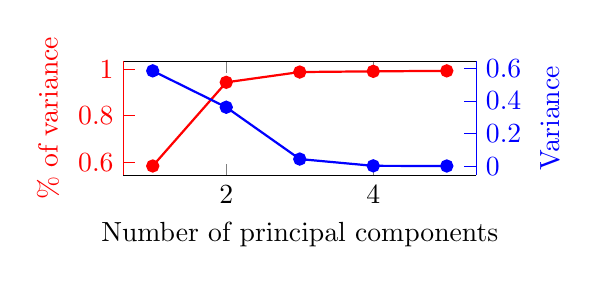
\begin{tikzpicture}
    \begin{axis}[width=0.5\textwidth,height=0.25\textwidth,ylabel=\% of variance,xlabel=Number of principal components,axis y line*=left,yticklabel style=red,ylabel style=red, y axis line style=red,ytick style=red]
      \addplot[thick,mark=*,red] coordinates { (1,0.58318064)  (2,0.94418758)  (3,0.98856319)  (4,0.99157161)  (5,0.99366953)};
    \end{axis}
    \begin{axis}[width=0.5\textwidth,height=0.25\textwidth,axis y line*=right,axis x line=none,ylabel=Variance,yticklabel style=blue,ylabel style=blue, y axis line style=blue,ytick style=blue]
      \addplot[thick,mark=*,blue] coordinates { (1,0.58318064)  (2,0.36100695)  (3,0.04437561)  (4,0.00300841)  (5,0.00209792)};
    \end{axis}
  \end{tikzpicture}
\end{center}
\item Principal components
\begin{center}
  \begin{tikzpicture}
    \begin{axis}[width=0.9\textwidth,height=0.3\textwidth,grid,xmin=400,xmax=900,cycle list name=color list]
      \addplot+[thick] table[col sep=comma,x index=0,y index=1] {figures/pca_pcs.csv};
      \addplot+[thick] table[col sep=comma,x index=0,y index=2] {figures/pca_pcs.csv};
      \addplot+[thick] table[col sep=comma,x index=0,y index=3] {figures/pca_pcs.csv};
      \legend{pc1,pc2,pc3};
    \end{axis}
  \end{tikzpicture}
\end{center}
\end{itemize}
\end{frame}
\begin{frame}[fragile,label={sec:org342cada}]{PCA case study 3/3}
 \begin{minted}[fontsize=\footnotesize,obeytabs=true,tabsize=4,bgcolor=bg]{python}
# Projection of the first PCs
imp = sp.dot(im,pca.components_[:3,:].T)
imp.shape = (h,w,3)

# Save image
rt.write_data('../Data/pca_university.tif',imp,GeoT,Proj)
\end{minted}
\begin{columns}
\begin{column}{0.3\columnwidth}
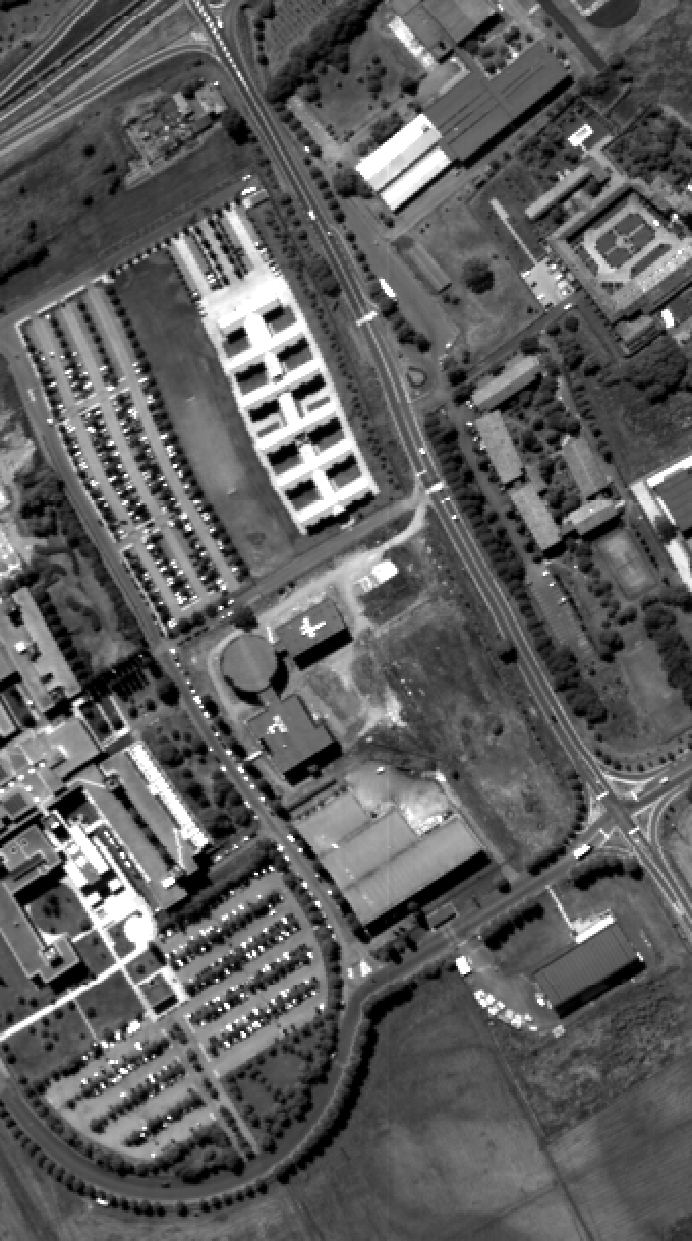
\includegraphics[width=0.75\linewidth]{./figures/university_pc1.png}
\end{column}

\begin{column}{0.3\columnwidth}
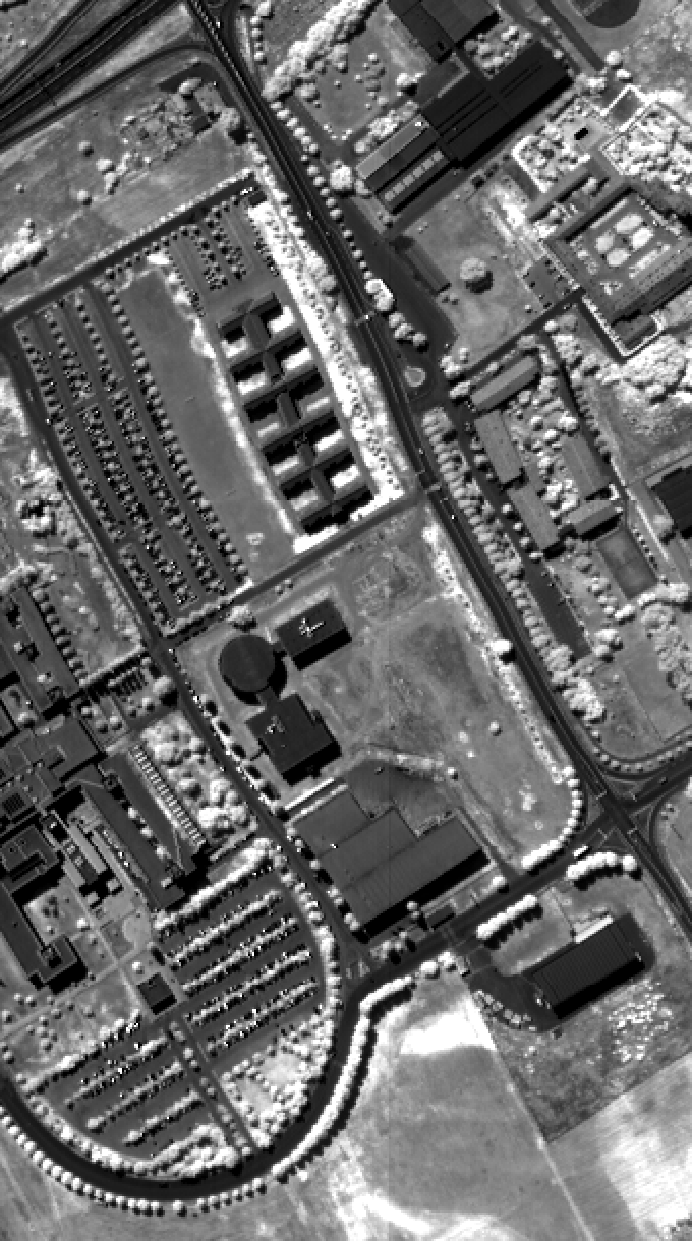
\includegraphics[width=0.75\linewidth]{./figures/university_pc2.png}
\end{column}

\begin{column}{0.3\columnwidth}
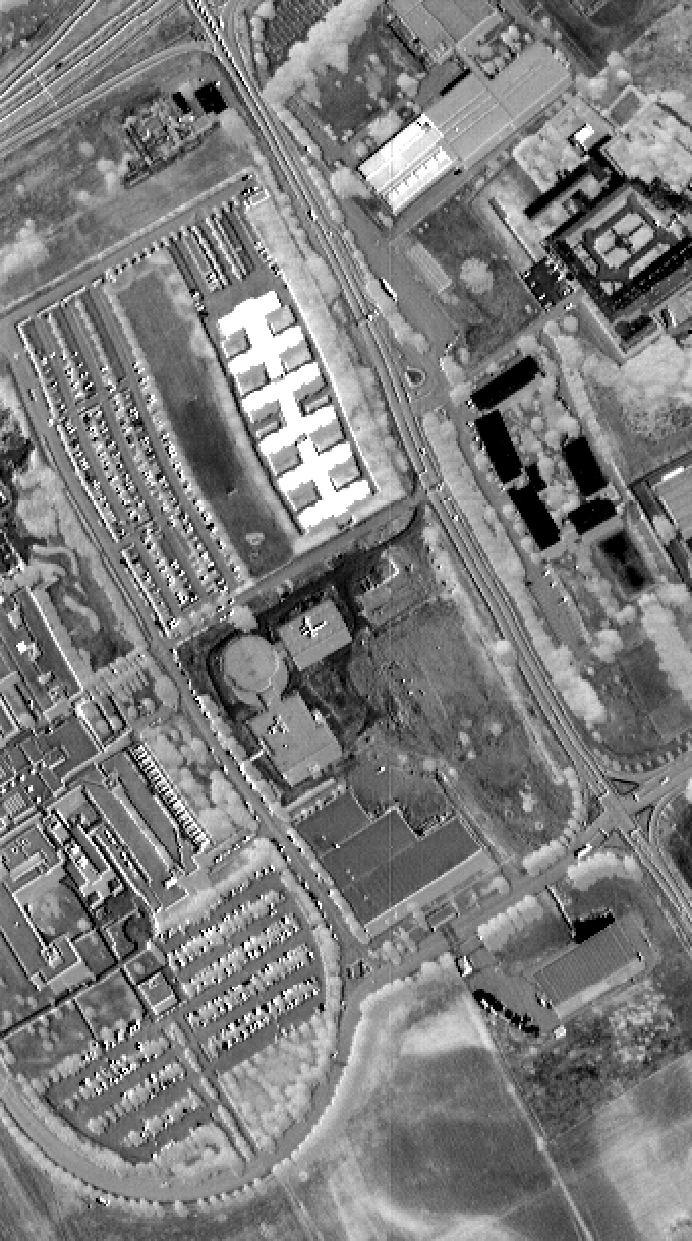
\includegraphics[width=0.75\linewidth]{./figures/university_pc3.png}
\end{column}
\end{columns}
\end{frame}

\begin{frame}[label={sec:org33c8b50}]{Kernel PCA}
\begin{itemize}
\item PCA is limited to second order information
\item To capture higher-order statistics, it is possible to map the data onto another space \(\mathcal{H}\)
\begin{eqnarray*}
  \begin{array}{rcl}
    \phi:\mathbb{R}^d &\to&\mathcal{H}\\
    \mathbf{x}&\mapsto&\phi(\mathbf{x}).
  \end{array}
\end{eqnarray*}
\item In \(\mathcal{H}\), conventional PCA can be applied.
\item Using the \emph{kernel trick} it is possible to directly work on the \emph{kernel matrix} in \(\mathbb{R}^d\)
\begin{eqnarray*}\label{kpca:matrix}
 \mathbf{K}=\left(
 \begin{array}{cccc}
 k(\mathbf{x}_1,\mathbf{x}_1) & k(\mathbf{x}_1,\mathbf{x}_2) & \ldots & k(\mathbf{x}_1,\mathbf{x}_n)\\
 k(\mathbf{x}_2,\mathbf{x}_1) & k(\mathbf{x}_2,\mathbf{x}_2) & \ldots & k(\mathbf{x}_2,\mathbf{x}_n)\\ 
 \vdots & \vdots & \ddots & \vdots \\
 k(\mathbf{x}_n,\mathbf{x}_1) & k(\mathbf{x}_n,\mathbf{x}_2) & \ldots & k(\mathbf{x}_n,\mathbf{x}_n)\\
 \end{array}\right).
\end{eqnarray*}
\item <2> KPCA versus PCA:

\begin{center}
  \begin{tabular}{ccc}
  \begin{tikzpicture}
    \begin{axis}[width=0.3\textwidth,height=0.3\textwidth,grid]
      \addplot[scatter,only marks,scatter src=explicit] table[col sep =comma,meta index=2,x index=0,y index=1] {figures/kpca_data.csv};
    \end{axis}
  \end{tikzpicture}&
  \begin{tikzpicture}
    \begin{axis}[width=0.3\textwidth,height=0.3\textwidth,grid]
      \addplot[scatter,only marks,scatter src=explicit] table[col sep =comma,meta index=2,x index=0,y index=1] {figures/kpca_datap.csv};
    \end{axis}
  \end{tikzpicture}&
                     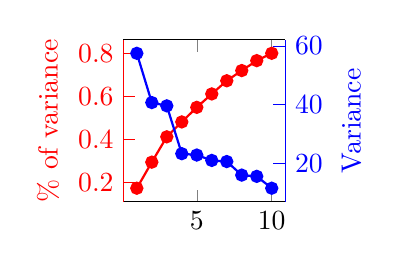
\begin{tikzpicture}
      \begin{axis}[width=0.3\textwidth,height=0.3\textwidth,ylabel=\% of variance,axis y line*=left,yticklabel style=red,ylabel style=red, y axis line style=red,ytick style=red]
        \addplot[thick,mark=*,red] coordinates { (1,0.171950045779)
          (2,0.293633371022)
          (3,0.41194893578)
          (4,0.481444806977)
          (5,0.54956124474)
          (6,0.612183510855)
          (7,0.673659036749)
          (8,0.721296411495)
          (9,0.767653893262)
          (10,0.80191080235)};
      \end{axis}
      \begin{axis}[width=0.3\textwidth,height=0.3\textwidth,axis y line*=right,axis x line=none,ylabel=Variance,yticklabel style=blue,ylabel style=blue, y axis line style=blue,ytick style=blue]
        \addplot[thick,mark=*,blue] coordinates {(1,57.4446834929)
          (2,40.6516908637)
          (3,39.5265970358)
          (4,23.2170239146)
          (5,22.7561859043)
          (6,20.9207054308)
          (7,20.5376050443)
          (8,15.914586718)
          (9,15.4870029584)
          (10,11.4444709279) };
      \end{axis}
    \end{tikzpicture}         
  \end{tabular}

\end{center}
\end{itemize}
\end{frame}

\begin{frame}[label={sec:orgc34857e}]{Kernel PCA in practice}
\begin{itemize}
\item Choose the kernel and its parameters
\item Compute the kernel matrix \(\mathbf{K}\) for all the pixels (or a subset)
\item Center the matrix
\begin{eqnarray*}
 \mathbf{K}_c=\mathbf{K}-\mathbf{1}_n\mathbf{K}-\mathbf{K}\mathbf{1}_n+\mathbf{1}_n\mathbf{K}\mathbf{1}_n
\end{eqnarray*}
\item Solve the eigenproblems
\begin{eqnarray*}
  \lambda\boldsymbol{\alpha}=\mathbf{K}\boldsymbol{\alpha} \text{ subject to } \|\boldsymbol{\alpha}\|_2 = \frac{1}{\lambda}
\end{eqnarray*}
\item Project on the \(p\) first \emph{kernel principal components}: \(\phi^{kpc}(\mathbf{x})=\begin{bmatrix}\phi^{kpc}_1(\mathbf{x})&\hdots&\phi^{kpc}_p(\mathbf{x})\end{bmatrix}^t\)
\begin{eqnarray*}
  \phi^{kpc}_j(\mathbf{x})=\sum_{i=1}^n \alpha_{ki} k(\mathbf{x}_i,\mathbf{x})
\end{eqnarray*}
\end{itemize}
\end{frame}

\begin{frame}[fragile,label={sec:org11b911a}]{KPCA case study 1/3}
 From \cite{fauvel2009kernel}.

\begin{minted}[fontsize=\footnotesize,obeytabs=true,tabsize=4,bgcolor=bg]{python}
import rasterTools as rt
import scipy as sp
from sklearn.decomposition import KernelPCA
import matplotlib.pyplot as plt
from sklearn.preprocessing import StandardScaler

# Load data set
im,GeoT,Proj = rt.open_data('../Data/university.tif')
[h,w,b]=im.shape
im.shape=(h*w,b)
wave = sp.loadtxt('../Data/waves.csv',delimiter=',')

# Scale data
sc = StandardScaler()
im = sc.fit_transform(im)

# Do KPCA
kpca = KernelPCA(kernel='rbf',gamma=1.0/b,n_jobs=-1)
kpca.fit(im[::50,:]) # Use a subset of the total number of pixels
\end{minted}
\end{frame}
\begin{frame}[label={sec:orga4abf28}]{KPCA case study 2/3}
\begin{itemize}
\item Explained variance
\begin{center}
  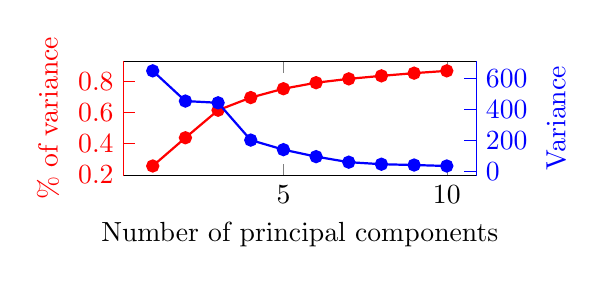
\begin{tikzpicture}
    \begin{axis}[width=0.5\textwidth,height=0.25\textwidth,ylabel=\% of variance,xlabel=Number of principal components,axis y line*=left,yticklabel style=red,ylabel style=red, y axis line style=red,ytick style=red]
      \addplot[thick,mark=*,red] coordinates {(1,0.257631571125)
      (2,0.438129567049)
      (3,0.61420975716)
      (4,0.695091757082)
      (5,0.751533118467)
      (6,0.790148033382)
      (7,0.814644462352)
      (8,0.833924207631)
      (9,0.851128186791)
      (10,0.865878267501) };
    \end{axis}
    \begin{axis}[width=0.5\textwidth,height=0.25\textwidth,axis y line*=right,axis x line=none,ylabel=Variance,yticklabel style=blue,ylabel style=blue, y axis line style=blue,ytick style=blue]
      \addplot[thick,mark=*,blue] coordinates {(1,649.766197024)
      (2,455.229519695)
      (3,444.087481204)
      (4,203.990486367)
      (5,142.349357966)
      (6,97.389719371)
      (7,61.7818360658)
      (8,48.6249674864)
      (9,43.3897292304)
      (10,37.2008127987) };
      \end{axis}
  \end{tikzpicture}
\end{center}
\item Principal components
\begin{center}
  \begin{tikzpicture}
    \begin{axis}[width=0.9\textwidth,height=0.3\textwidth,grid,cycle list name=color list,xmin=0,xmax=4148]
      \addplot+[thick] table[col sep=comma,x index=0,y index=1] {figures/kpca_pcs.csv};
      \addplot+[thick] table[col sep=comma,x index=0,y index=2] {figures/kpca_pcs.csv};
      \addplot+[thick] table[col sep=comma,x index=0,y index=3] {figures/kpca_pcs.csv};
      \legend{kpc1,kpc2,kpc3};
    \end{axis}
  \end{tikzpicture}
\end{center}
\end{itemize}
\end{frame}
\begin{frame}[fragile,label={sec:orge474be2}]{KPCA case study 3/3}
 \begin{minted}[fontsize=\footnotesize,obeytabs=true,tabsize=4,bgcolor=bg]{python}
imp = kpca.transform(im)[:,:3]
imp.shape = (h,w,3)

# Save image
rt.write_data('../Data/kpca_university.tif',imp,GeoT,Proj)
\end{minted}
\begin{columns}
\begin{column}{0.3\columnwidth}
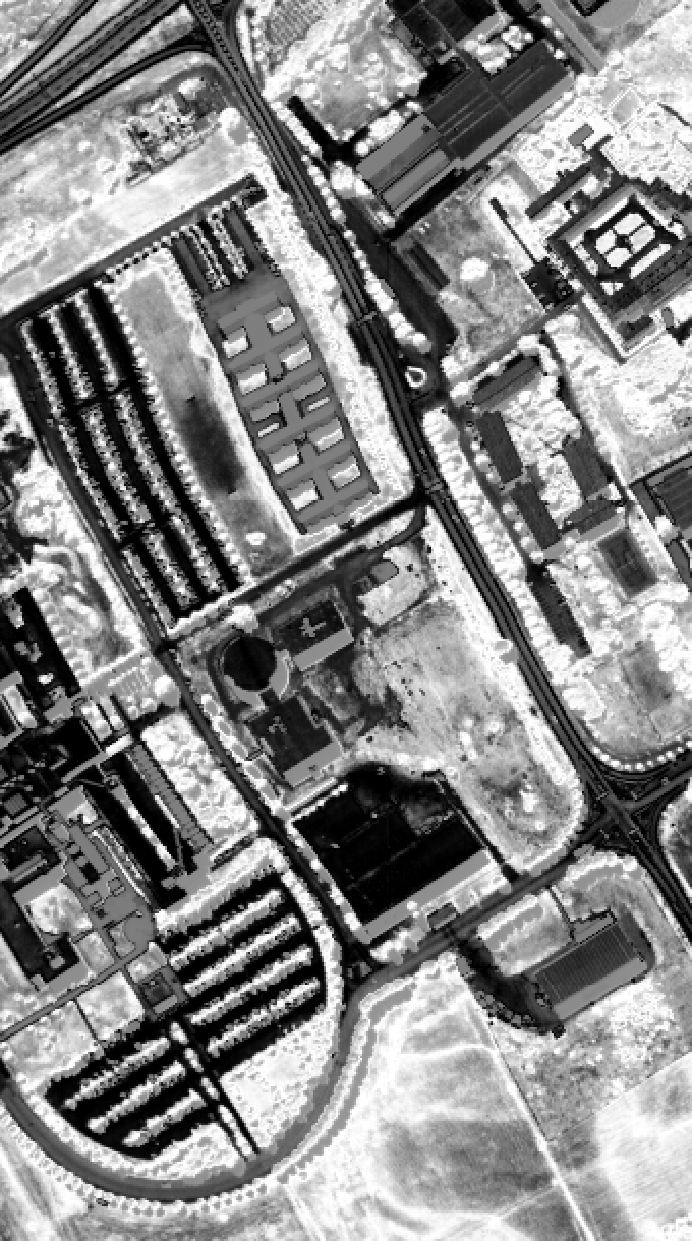
\includegraphics[width=0.75\linewidth]{./figures/university_kpc1.png}
\end{column}

\begin{column}{0.3\columnwidth}
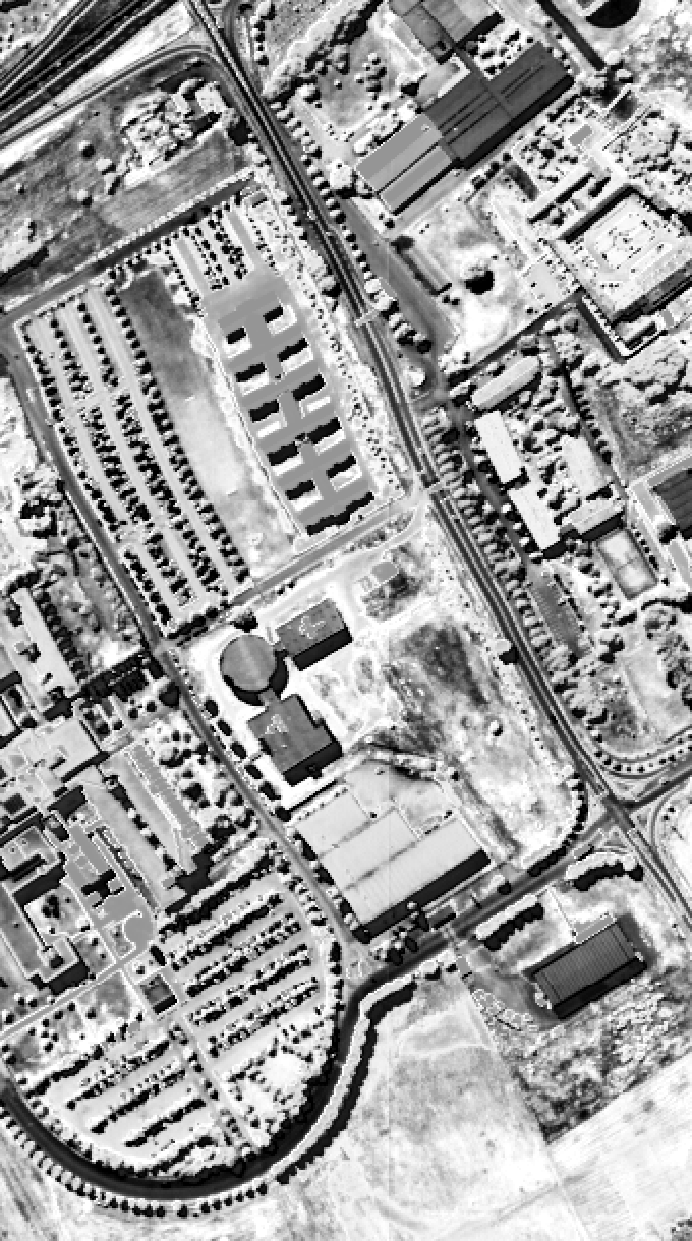
\includegraphics[width=0.75\linewidth]{./figures/university_kpc2.png}
\end{column}

\begin{column}{0.3\columnwidth}
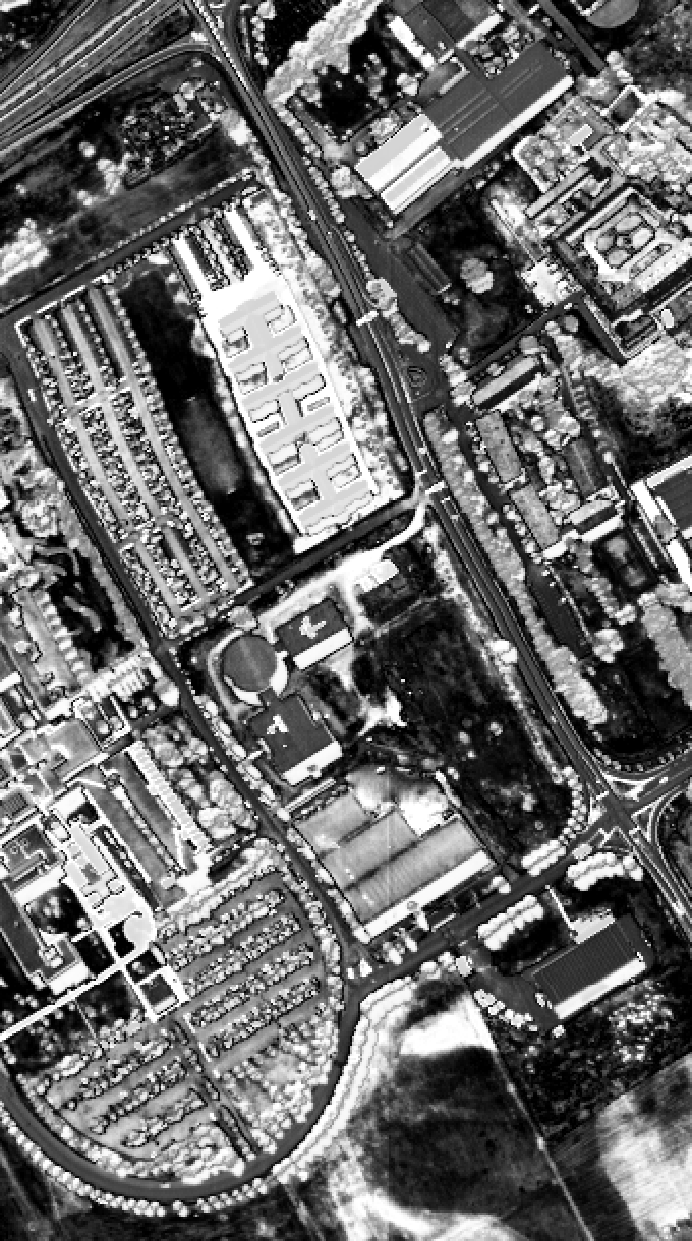
\includegraphics[width=0.75\linewidth]{./figures/university_kpc3.png}
\end{column}
\end{columns}
\end{frame}

\subsection{Supervised}
\label{sec:orgd79032b}
\begin{frame}[label={sec:org2454406}]{Fisher's Discriminant Analysis}
\begin{itemize}
\item We observe some \(\{\mathbf{x}_i,y_i\}_{i=1}^n\)
\item Use the label information to find the linear features that highlight differences among classes

\begin{center}
  \begin{tikzpicture}
    \begin{axis}[width=0.6\textwidth,grid,small,xmin=-5,xmax=5,ymin=-5,ymax=5]
      \addplot[scatter, only marks,scatter src=explicit]table[col sep=comma,meta index=2,x index =0,y index=1] {figures/lda_data.csv};      
      \addplot[domain=-5:5,very thick] {-x/0.52306077251960925*0.85229538790913895 - 3.65687201/3.04406312};
    \end{axis}
  \end{tikzpicture}
\end{center}
\item FDA: find \(\mathbf{a}\) such as the ratio between the \emph{between projected variance} and the \emph{sample projected variance} is maximal
\end{itemize}
\end{frame}
\begin{frame}[label={sec:org4d75b46}]{FDA Algorithm}
\begin{itemize}
\item Between-class covariance matrix:
\begin{eqnarray*}
  \mathbf{B} = \frac{1}{n}\sum_{c=1}^Cn_c(\boldsymbol{\mu}_c-\boldsymbol{\mu})(\boldsymbol{\mu}_c-\boldsymbol{\mu})^\top
\end{eqnarray*}
\item Sample covariance matrix
\begin{eqnarray*}
  \boldsymbol{\Sigma} = \frac{1}{n-1}\sum_{i=1}^n(\mathbf{x}_i-\boldsymbol{\mu})(\mathbf{x}_i-\boldsymbol{\mu})^\top
\end{eqnarray*}
\item The Fisher discriminant subspace is given by the eigenvectors of \(\boldsymbol{\Sigma}^{(-1)}\mathbf{B}\)
\item Remark: there are at most \(C-1\) eigenvectors because \(\text{Rank}(\mathbf{B})\leq C-1\).
\end{itemize}
\end{frame}
\begin{frame}[fragile,label={sec:org406677e}]{FDA case study 1/3}
 \begin{minted}[fontsize=\footnotesize,obeytabs=true,tabsize=4,bgcolor=bg]{python}
import rasterTools as rt
import scipy as sp
from sklearn.discriminant_analysis import LinearDiscriminantAnalysis

# Load data set
X,y=rt.get_samples_from_roi('../Data/university.tif','../Data/university_gt.tif')
wave = sp.loadtxt('../Data/waves.csv',delimiter=',')

# Select the same number of samples
nt = 900
xt,yt=[],[]
for i in sp.unique(y):
    t = sp.where(y==i)[0]
    nc = t.size
    rp =  sp.random.permutation(nc)
    xt.extend(X[t[rp[0:nt]],:])
    yt.extend(y[t[rp[0:nt]]])

xt = sp.asarray(xt)
yt = sp.asarray(yt)

# Do LDA
lda = LinearDiscriminantAnalysis(solver='eigen',shrinkage='auto')
lda.fit(xt,yt.ravel())
\end{minted}
\end{frame}
\begin{frame}[label={sec:orga51fee7}]{FDA case study 2/3}
\begin{itemize}
\item Projection on Fisher components
\begin{center}
  \begin{tabular}{cc}
 \begin{tikzpicture}
      \begin{axis}[width=0.4\textwidth,height=0.3\textwidth,xticklabels={,,},yticklabels={,,},grid,xlabel=FC 1,ylabel=FC 2]
        \addplot[scatter,only marks,scatter src=explicit,opacity=0.5] table[col sep =comma,meta index=4,x index=0,y index=1] {figures/lda_proj.csv};
      \end{axis}
    \end{tikzpicture}&
                       \begin{tikzpicture}
                         \begin{axis}[width=0.4\textwidth,height=0.3\textwidth,xticklabels={,,},yticklabels={,,},grid,,xlabel=FC 3,ylabel=FC 4]
                           \addplot[scatter,only marks,scatter src=explicit,opacity=0.5] table[col sep =comma,meta index=4,x index=3,y index=2] {figures/lda_proj.csv};
                         \end{axis}
                       \end{tikzpicture}
  \end{tabular}
\end{center}
\item Fisher components
\begin{center}
  \begin{tikzpicture}
    \begin{axis}[width=0.9\textwidth,height=0.3\textwidth,grid,xmin=400,xmax=900,cycle list name=color list]
      \addplot+[thick] table[col sep=comma,x index=0,y index=1] {figures/lda_pcs.csv};
      \addplot+[thick] table[col sep=comma,x index=0,y index=2] {figures/lda_pcs.csv};
      \addplot+[thick] table[col sep=comma,x index=0,y index=3] {figures/lda_pcs.csv};
      \legend{pc1,pc2,pc3};
    \end{axis}
  \end{tikzpicture}
\end{center}
\end{itemize}
\end{frame}
\begin{frame}[fragile,label={sec:orgd338d07}]{FDA case study 3/3}
 \begin{minted}[fontsize=\footnotesize,obeytabs=true,tabsize=4,bgcolor=bg]{python}
im,GeoT,Proj = rt.open_data('../Data/university.tif')
[h,w,b]=im.shape
im.shape=(h*w,b)
imp = lda.transform(im)[:,:3]
imp.shape = (h,w,3)
# Save image
rt.write_data('../Data/lda_university.tif',imp,GeoT,Proj)
\end{minted}
\begin{columns}
\begin{column}{0.3\columnwidth}
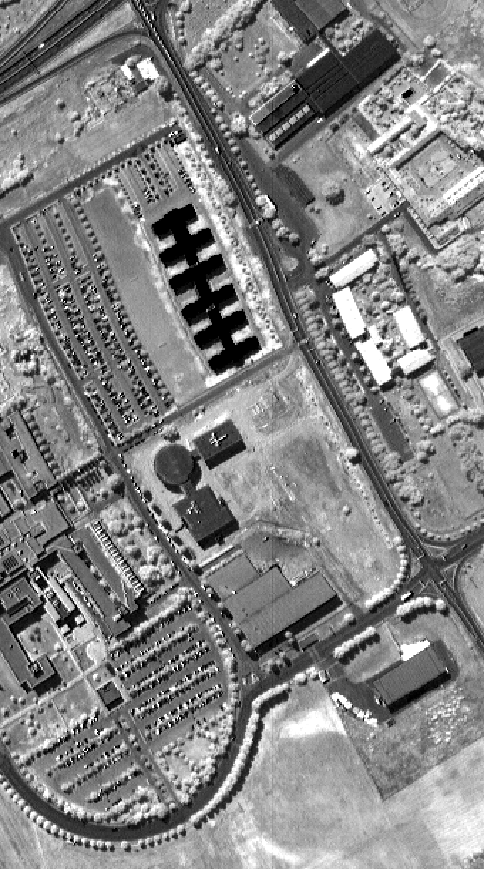
\includegraphics[width=0.75\linewidth]{./figures/university_lda1.png}
\end{column}

\begin{column}{0.3\columnwidth}
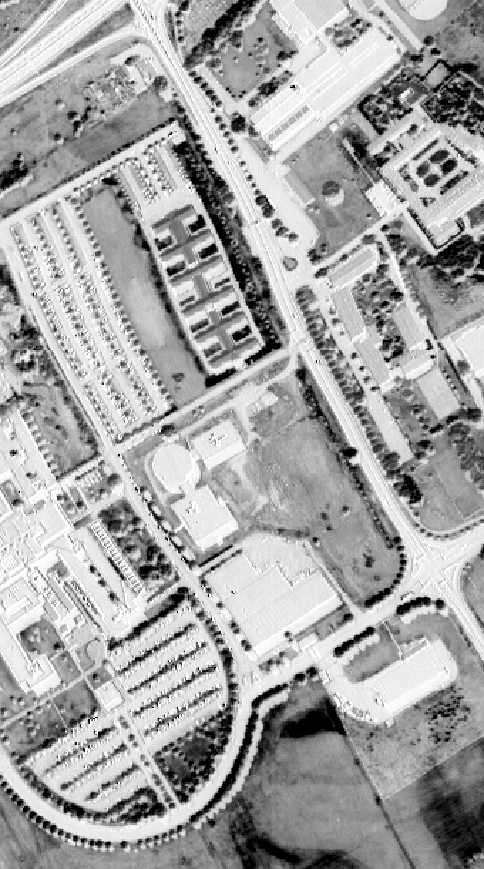
\includegraphics[width=0.75\linewidth]{./figures/university_lda2.png}
\end{column}

\begin{column}{0.3\columnwidth}
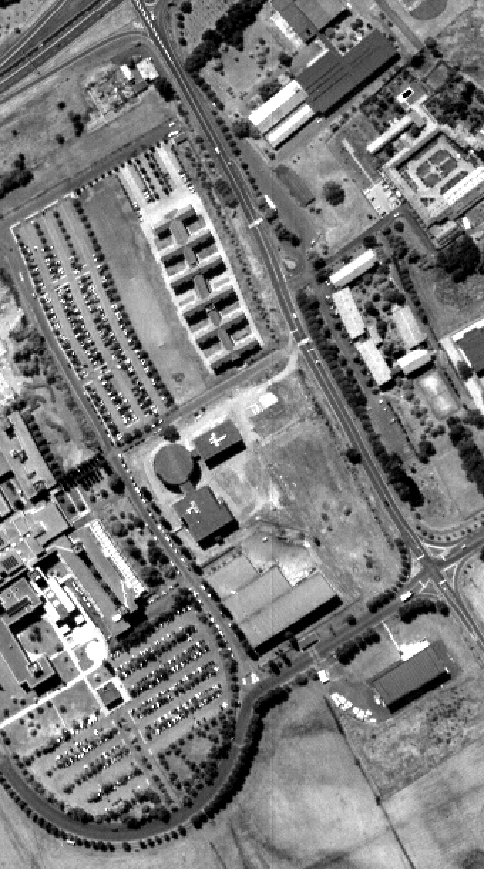
\includegraphics[width=0.75\linewidth]{./figures/university_lda3.png}
\end{column}
\end{columns}
\end{frame}

\begin{frame}[label={sec:org71ab952}]{Feature selection}
\begin{itemize}
\item Feature selection: pick few features \emph{from} the original ones (no combination)
\item In general, for feature selection, we need:
\begin{itemize}
\item \emph{Criterion} to evaluate how perform the model with a given subset
\item \emph{Optimization   procedure}   to  find   the   subset   that  minimizes/maximizes the criterion
\end{itemize}
\item For instance:   
\begin{center}
\begin{tabular}{lll}
\toprule
Criterion & Optimization & Ref.\\
\midrule
Entropy & Genetic algorithm & \cite{chein2007hyperspectral}\\
Jeffries Matusita & Exhaustive Search & \cite{4069122}\\
Classification error & Forward search/GA & \cite{lebris:fs,7847352}\\
\(\ell_1\) norm & Linear-SVM & \cite{tuia2014automatic}\\
\bottomrule
\end{tabular}
\end{center}
\end{itemize}
\end{frame}

\begin{frame}[label={sec:org69e03a0}]{Large scale feature selection with GMM}
\begin{itemize}
\item Fast  forward strategy  based  on  a nonlinear  model  driven by  an
estimate of the classification error or a measure of separability:
\begin{center}
\begin{tabular}{lll}
\toprule
Criterion & Type & Complexity\\
\midrule
Overall accuracy & Accuracy & High\\
Cohen's kappa & Accuracy & High\\
F1 mean & Accuracy & High\\
\midrule
Kullback-Leibler divergences & Divergence & Low\\
Jeffries-Matusita distance & Divergence & Low\\
\bottomrule
\end{tabular}
\end{center}
\item Use \emph{Gaussian Mixture Models} (natural extension du multiclass problem)
\item Fast update and fast forward search \cite{7847352}: based on linear algebra
\end{itemize}
\end{frame}

\begin{frame}[label={sec:org7e03d4c}]{Algorithm 1/2}
The forward feature selection works as follow:
\begin{itemize}
\item Starts with an empty pool \(F\) of selected features,
\item Select the  feature \(f_1\) that  provides the best value  for the
selected criterion and add it to \(F\).
\item Select  the  feature \(f_2\)  such  that  the couple  of  features
\((f_1,f_2)\) provides  the best value for  the selected criterion
and add it to \(F\).
\item Select  the feature  \(f_3\)  such that  the  triplet of  features
\((f_1,f_2,f_3)\) \ldots{}
\item \ldots{}
\item The algorithm stops either if the increase of the criterion is too
low or if the maximum number of features is reached.
\end{itemize}
\end{frame}

\begin{frame}[label={sec:orgee0378f}]{Algorithm 2/2}
\tikzset{noeud/.style={minimum width=1.5cm,minimum height=1cm,text width = 1.25cm,text centered,rounded corners=1pt,draw,rectangle,thick}}
\tikzstyle{arrow}=[->,>=stealth,thick]
\tikzstyle{arrow2}=[dashed,->,>=stealth,thick]
\centerline{\resizebox{0.65\linewidth}{!}{\begin{tikzpicture}
    % Nodes
    \node[noeud] (S) at (0,0) {$\mathcal{S}$};
    \node[noeud] (S1) at (-4,-2) {$\mathcal{S}_1$};
    \node[noeud] (S2) at (-2,-2) {$\mathcal{S}_2$};
    \node[noeud] (S3) at (0,-2) {$\mathcal{S}_3$};
    \node[noeud] (S4) at (2,-2) {$\mathcal{S}_4$};
    \node[noeud,magenta] (S5) at (4,-2) {$\mathcal{S}_5$};
    \node[noeud] (model) at (-3,0) {Model};
    \node[noeud,orange] (update) at (-2,-4) {Update};
    \node[noeud,orange] (predict) at (2,-4) {OA($\lambda_i$)};
    %Arrows
    \draw[arrow] (S.south)|-(0,-1)-|(S1.north);
    \draw[arrow] (-2,-1)-|(S2.north);
    \draw[arrow] (0,-1)-|(S3.north);
    \draw[arrow] (2,-1)-|(S4.north);
    \draw[arrow] (0,-1)-|(S5.north);
    \draw[arrow] (S.west) -- (model.east);
    \draw[arrow2] (model.west) -| (-5,0) |- (-5,-4) -- (update.west);
    \draw[arrow] (S5.south) |- (2,-3) -| (update.north);
    \draw[arrow2] (update.east) -- (predict.west);
    \draw[arrow] (2,-3) -- (predict.north);
    \draw[dotted,->,>=stealth,thick] (predict.south) -- (2,-5);
    \node (plot) at (-0.7,-7.8) {\begin{axis}[x tick label style={rotate=45,anchor=east},grid,xmin=430,xmax=860,xlabel=$\lambda_i$,ylabel=OA,footnotesize]
        \addplot[thick,smooth] table[x=var,y=error,col sep=comma]  {figures/kcv_1.csv};
      \end{axis}};
\end{tikzpicture}}}
\end{frame}

\begin{frame}[fragile,label={sec:org9392a2d}]{FFFS case study 1/3}
 \begin{minted}[fontsize=\footnotesize,obeytabs=true,tabsize=4,bgcolor=bg]{python}
import rasterTools as rt
import scipy as sp
import npfs as npfs

# Load data set
X,y=rt.get_samples_from_roi('../Data/university.tif','../Data/university_gt.tif')
wave = sp.loadtxt('../Data/waves.csv',delimiter=',') 

# Select the same number of samples
nt = 900
xt,yt=[],[]
for i in sp.unique(y):
    t = sp.where(y==i)[0]
    nc = t.size
    rp =  sp.random.permutation(nc)
    xt.extend(X[t[rp[0:nt]],:])
    yt.extend(y[t[rp[0:nt]]])

xt = sp.asarray(xt)
yt = sp.asarray(yt)

# Do FFFS
maxVar = 12
model = npfs.GMMFeaturesSelection()
model.learn_gmm(xt,yt)
idx, crit, [] = model.selection('forward',xt, yt,criterion='kappa', varNb=maxVar, nfold=5)
\end{minted}
\end{frame}

\begin{frame}[label={sec:org8c4d418}]{FFFS case study 2/3}
\begin{itemize}
\item Criterion
  \begin{center}
      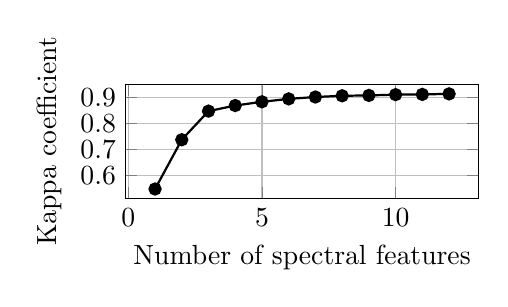
\begin{tikzpicture}
        \begin{axis}[width=0.5\textwidth,height=0.25\textwidth,ylabel=Kappa coefficient,xlabel=Number of spectral features,grid]
          \addplot[thick,mark=*,] coordinates {(1,0.546805555556)
(2,0.736944444444)
(3,0.847361111111)
(4,0.868888888889)
(5,0.883333333333)
(6,0.894583333333)
(7,0.901805555556)
(8,0.906527777778)
(9,0.907916666667)
(10,0.910972222222)
(11,0.911805555556)
(12,0.913888888889)};
        \end{axis}
      \end{tikzpicture}
    \end{center}
\item Mean projection on best bands
\end{itemize}


\begin{center}
\begin{tikzpicture}                           
\begin{axis}[width=0.4\textwidth,height=0.3\textwidth,xticklabels={,,},yticklabels={,,},grid,xlabel={$\hat{\lambda}_1 = 555$},ylabel={$\hat{\lambda}_2 = 798$}]
\addplot[scatter,only marks,scatter src=explicit] table[col sep =comma, meta index=2,x index=0,y index=1] {figures/fffsMean.csv};
\end{axis}
\end{tikzpicture}
\end{center}
\end{frame}

\section{Spatial feature extaction}
\label{sec:org6dc64b8}
\begin{frame}[label={sec:orgabba0ee}]{Why spatial feature extraction?}
\centerline{\begin{tabular}{ccc}
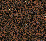
\includegraphics[width=0.2\linewidth]{figures/rgb_house_shuffle} & 
\includegraphics[width=0.2\linewidth]{figures/rgb_house_sort} & 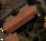
\includegraphics[width=0.2\linewidth]{figures/rgb_house_original}\\
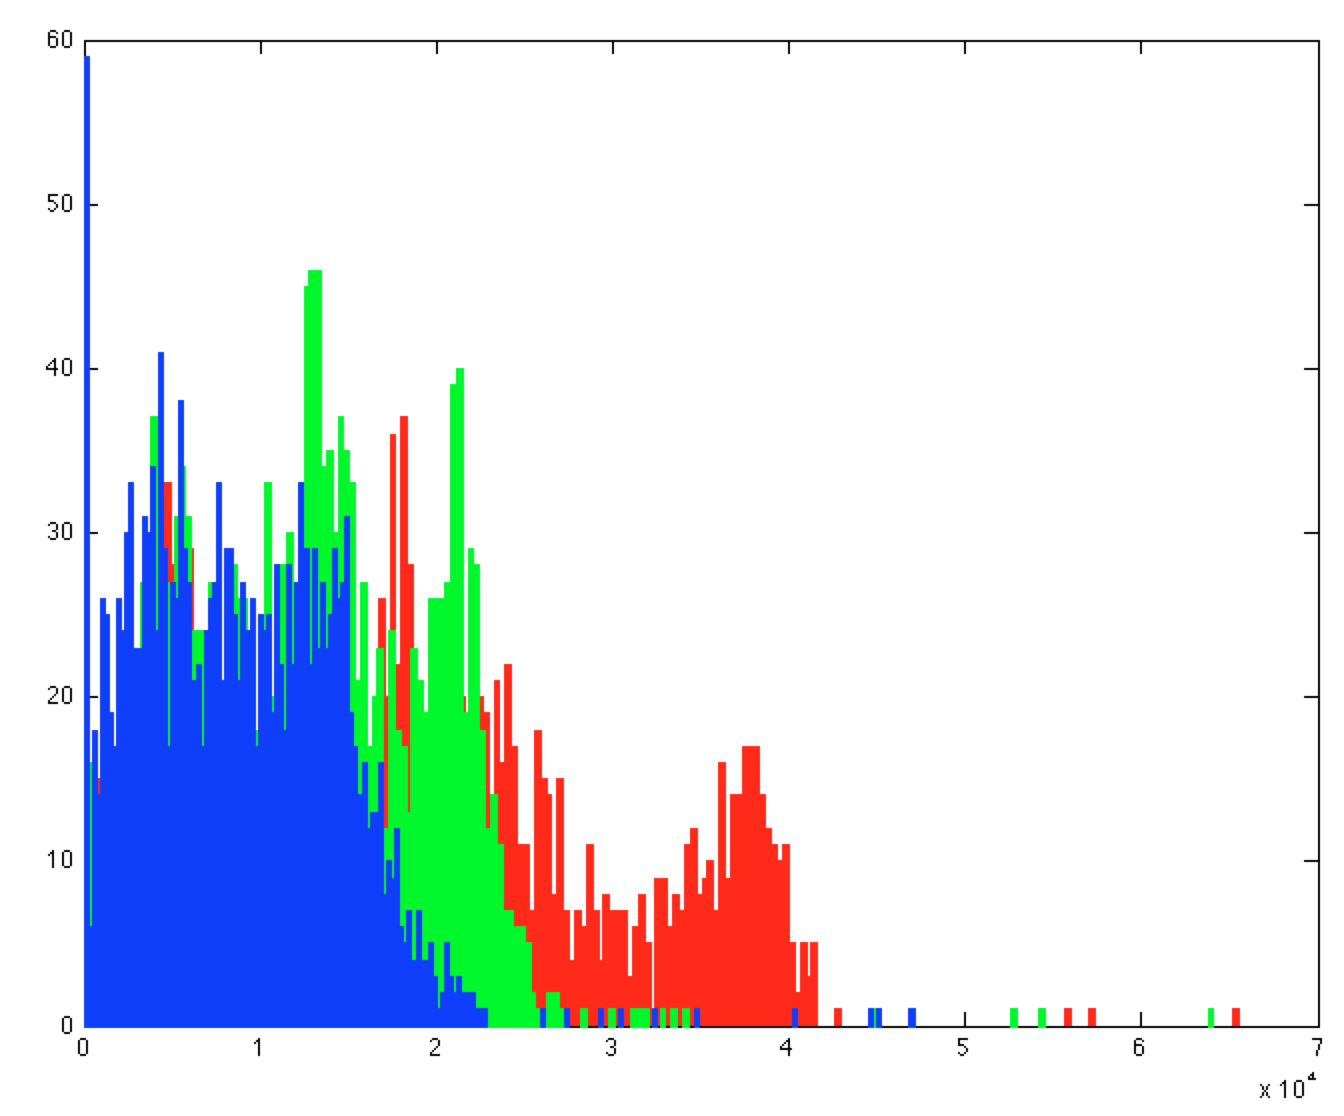
\includegraphics[width=0.2\linewidth]{figures/rgb_house_hist} & 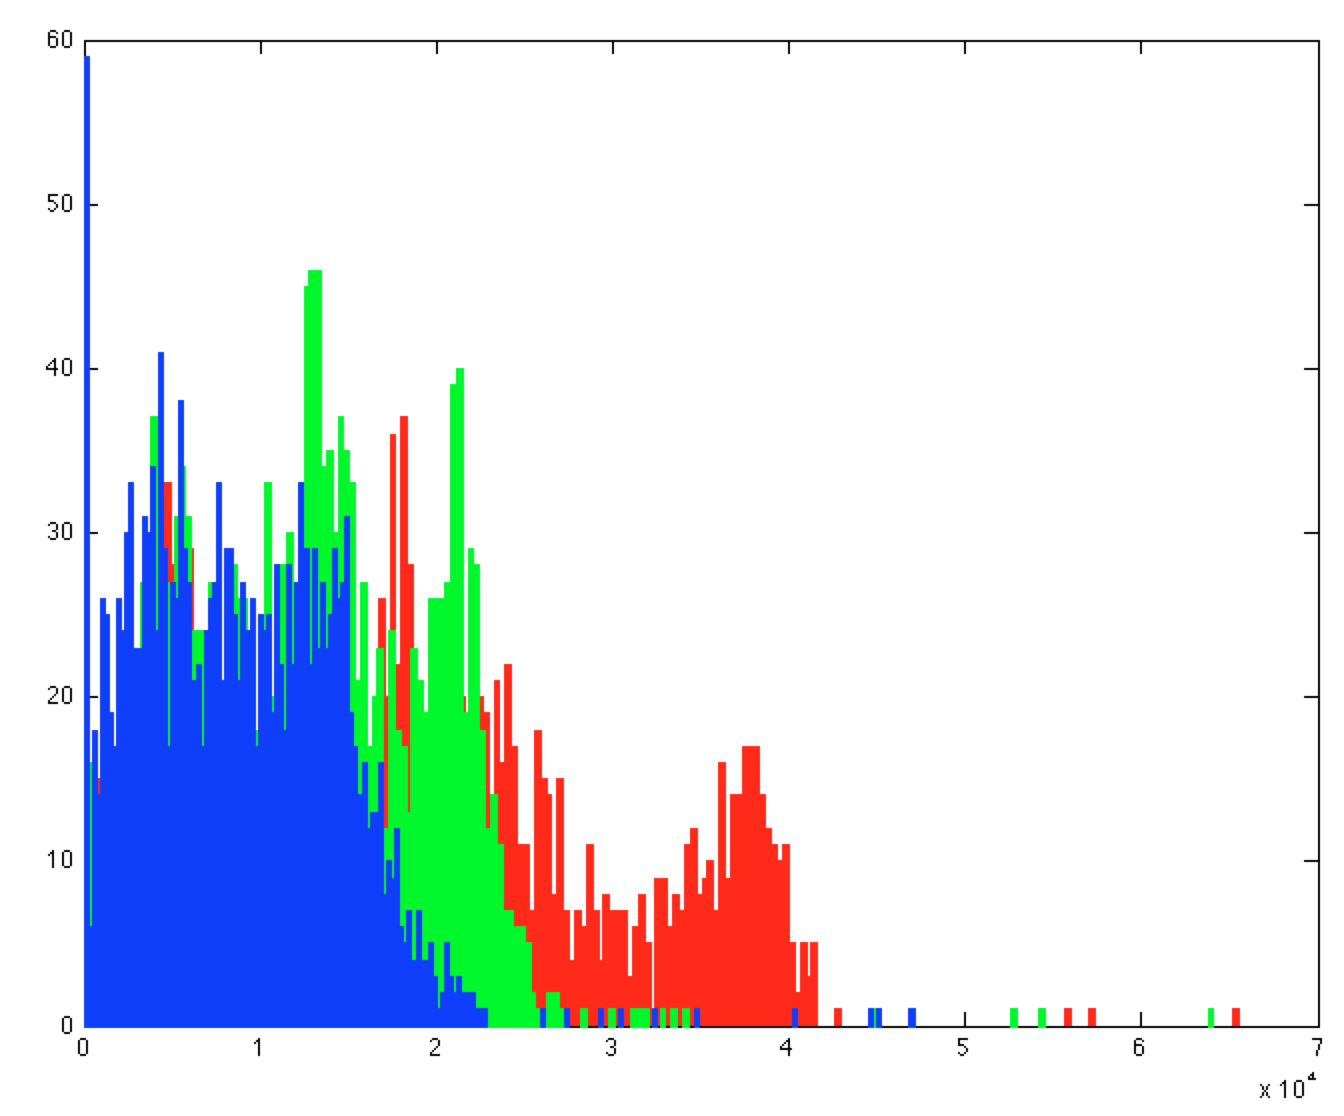
\includegraphics[width=0.2\linewidth]{figures/rgb_house_hist} & 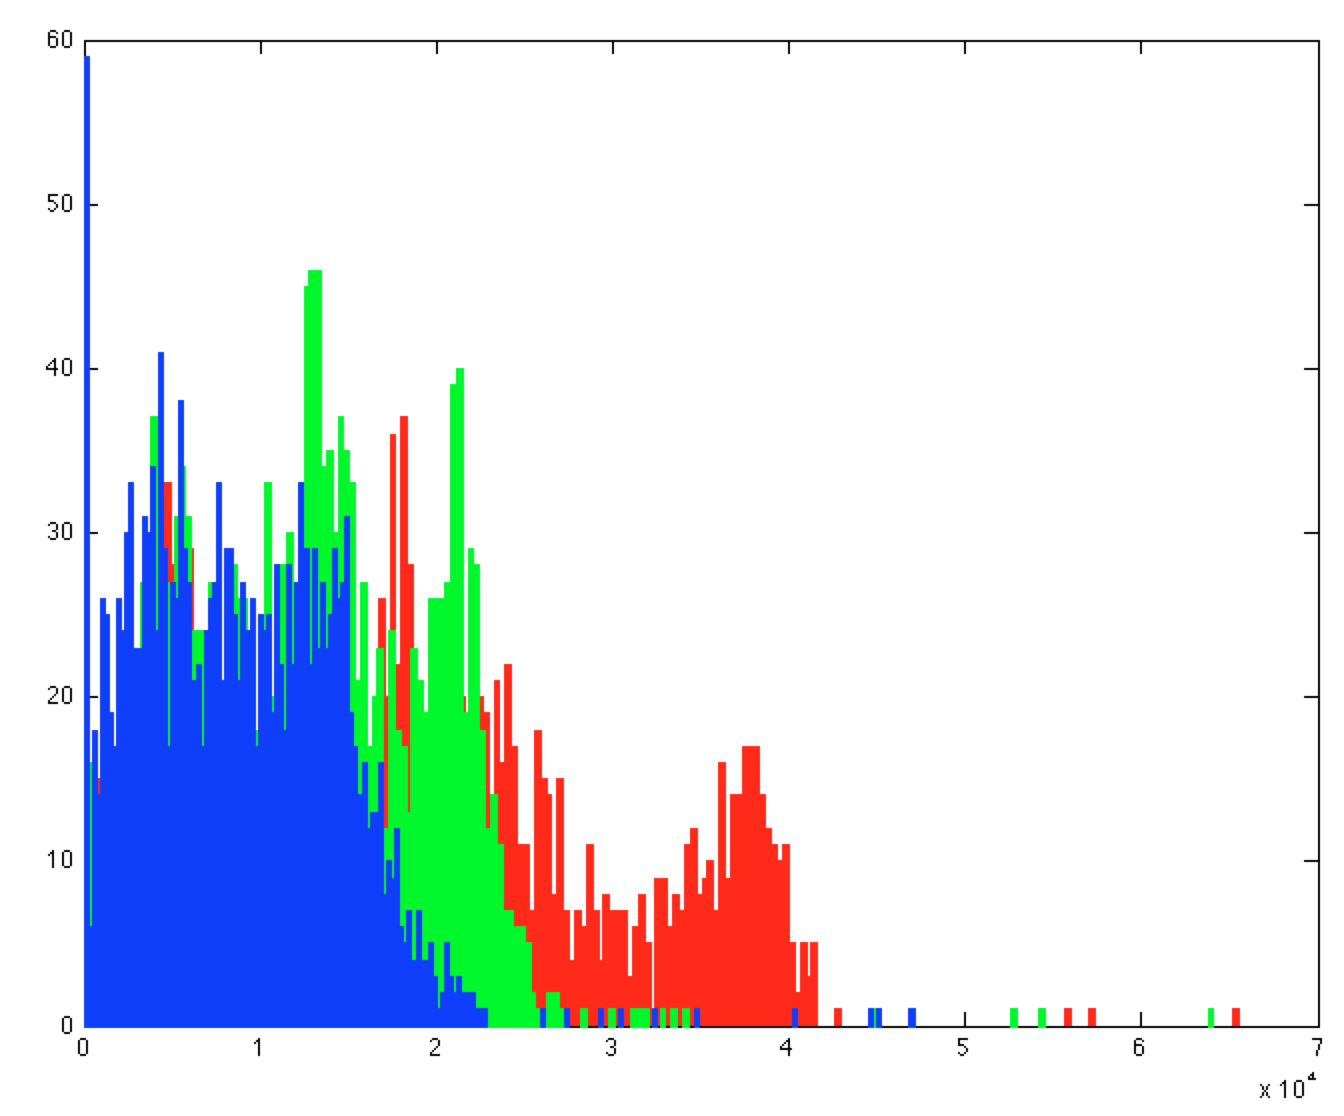
\includegraphics[width=0.2\linewidth]{figures/rgb_house_hist}
\end{tabular}}
\end{frame}

\subsection{Spatial filters}
\label{sec:org25ab728}
\begin{frame}[label={sec:orgfc01b00}]{Spatial neighborhood}
\begin{itemize}
\item The neighborhood of a given pixel is the set of pixels that are connected to it.
\item For a flat (grayscale) image :
\centerline{\newcounter{a}\newcounter{b}\begin{tikzpicture}
    \foreach \x in {1,...,3}
    \foreach \y in {1,...,3}
    { 
      \draw (\x,\y)+(-.5,-.5) rectangle ++(.5,.5);
      \pgfmathsetcounter{a}{\x-2}
      \pgfmathsetcounter{b}{2-\y}
      \draw (\x,\y) node{$\mathbf{x}_{\thea,\theb}$};
    }
    \draw[red,thick] (1.5,0.5) rectangle +(1,3);
    \draw[red,thick] (0.5,1.5) rectangle +(3,1);
    \draw (2,0) node{4-connected};
  \end{tikzpicture}\hspace{1cm}\begin{tikzpicture}
    \foreach \x in {1,...,3}
    \foreach \y in {1,...,3}
    { 
      \draw (\x,\y)+(-.5,-.5) rectangle ++(.5,.5);
      \pgfmathsetcounter{a}{\x-2}
      \pgfmathsetcounter{b}{2-\y}
      \draw (\x,\y) node{$\mathbf{x}_{\thea,\theb}$};
    }
    \draw[red,thick] (0.5,0.5) rectangle(3.5,3.5);
    \draw (2,0) node{8-connected};
  \end{tikzpicture}}
\item Wide range of processing are  based on pixel neighborhood
\begin{itemize}
\item De noising,
\item Texture analysis,
\item Edges detection,
\item Pattern recognition,
\item \ldots{}
\end{itemize}
\end{itemize}
\end{frame}
\begin{frame}[label={sec:org5f883fc}]{Template filters}
\uline{Steps}:
\begin{enumerate}
\item Define the template  \(G\): 4/8-connected and size
\item Define  the processing  \(f\) on the  neighborhood. If  \(f\) is linear \(\leftrightarrow\) convolution.
\item Scan all the pixels:
\end{enumerate}
$$\mathbf{x}_{ij}^f = f(\mathbf{x}_1,\ldots,\mathbf{x}_N),\ \mathbf{x}_n\in G(i,j)$$

\begin{center}
Max Filter
\end{center}
\centerline{\resizebox{0.5\textwidth}{!}{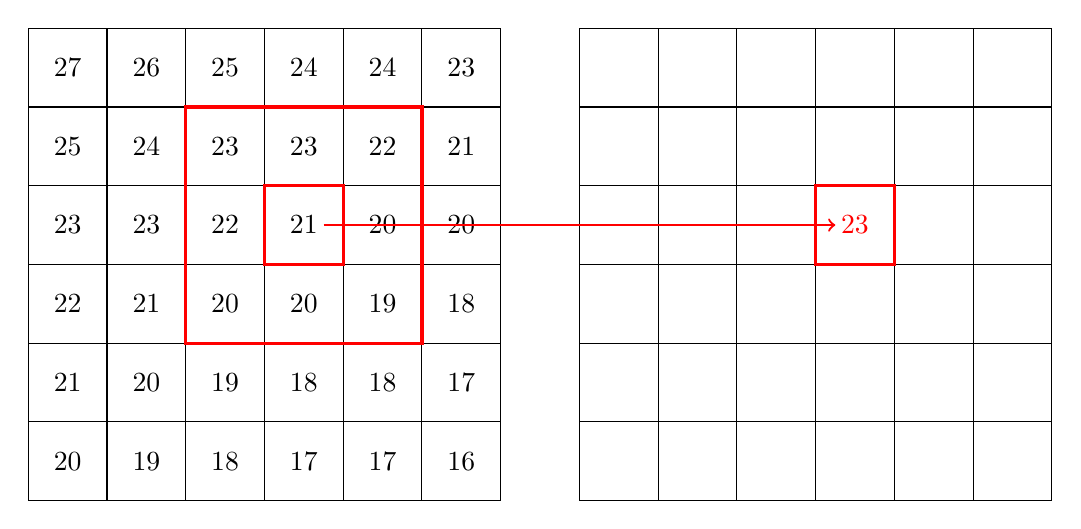
\begin{tikzpicture}
        \foreach \x in {1,...,6}
        \foreach \y in {1,...,6}
        {
          \draw (\x,\y)+(-.5,-.5) rectangle ++(.5,.5);
          \draw (\x,\y) node{\pgfmathparse{int(10*(exp(-\x/10) + exp(\y/10)))}\pgfmathresult};
        }
        \draw[help lines,red,very thick](3.5,3.5) rectangle +(1,1);
        \draw[help lines,red,very thick](2.5,2.5) rectangle +(3,3);
        \foreach \x in {1,...,6}
        \foreach \y in {1,...,6}
        {
          \draw (\x+7,\y)+(-.5,-.5) rectangle ++(.5,.5);
        }
        \draw[help lines,red,very thick](3.5+7,3.5) rectangle +(1,1);
        \draw[red,very thick](11,4) node{23};
        \draw[->,red,thick]  (4.25,4) -- (10.75,4);
      \end{tikzpicture}}}
\end{frame}
\begin{frame}[label={sec:org630093c}]{Some filters}
\begin{itemize}
\item G = \(\begin{bmatrix} 1 & 1  & 1 \\1 & 1  & 1 \\1 & 1  & 1 \end{bmatrix}\), for a \(3\times 3\) neighborhood.
\item Mean filter
$$\mathbf{x}^{m}(x,y) = \frac{1}{9}\sum_{i,j=-1}^1\mathbf{x}(x+i,y+j)$$
\item Variance filter:
$$\mathbf{x}^{v}(x,y) = \frac{1}{9}\sum_{i,j=-1}^1\big(\mathbf{x}(x+i,y+j)-\mathbf{x}^{m}(x,y)\big)^2$$
\item Range filter:
$$\mathbf{x}^{r}(x,y) = \max_{i,j\in G}[\mathbf{x}(x+i,y+j)] - \min_{i,j\in G}[\mathbf{x}(x+i,y+j)]$$
\item Median filter:
$$\mathbf{x}^{m}(x,y) = \text{median}_{i,j\in G}[\mathbf{x}(x+i,y+j)]$$
\end{itemize}
\end{frame}
\begin{frame}[fragile,label={sec:org1d5afec}]{Template filters in action 1/3}
 \begin{center}
\alert{For multidimensional images: Use spectral feature extraction to get flat images!} See \ref{sec:org1b2ae1b}
\end{center}

\begin{minted}[fontsize=\footnotesize,obeytabs=true,tabsize=4,bgcolor=bg]{sh}
# Compute the different filters with a template of size 3x3 and 11x11
for i in 3 11
do
    # Mean filter
    otbcli_BandMathX -il ../Data/pca_university.tif -out ../Data/pca_mean_${i}_${i}_university.tif \
		     -exp "mean(im1b1N${i}x${i}); mean(im1b2N${i}x${i}); mean(im1b3N${i}x${i})"

    # Var filter
    otbcli_BandMathX -il ../Data/pca_university.tif -out ../Data/pca_std_${i}_${i}_university.tif \
		     -exp "var(im1b1N${i}x${i}); var(im1b2N${i}x${i}); var(im1b3N${i}x${i})"

    # Range filter
    otbcli_BandMathX -il ../Data/pca_university.tif -out ../Data/pca_range_${i}_${i}_university.tif \
		     -exp "vmax(im1b1N${i}x${i})-vmin(im1b1N${i}x${i}); vmax(im1b2N${i}x${i})-vmin(im1b2N${i}x${i});\
                     vmax(im1b3N${i}x${i})-vmin(im1b3N${i}x${i})"

    # Median filter
    otbcli_BandMathX -il ../Data/pca_university.tif -out ../Data/pca_median_${i}_${i}_university.tif \
		     -exp "median(im1b1N${i}x${i}); median(im1b2N${i}x${i}); median(im1b3N${i}x${i})"
done
\end{minted}
\end{frame}

\begin{frame}[label={sec:orgdeacea0}]{Template filters in action 2/3}
\begin{center}
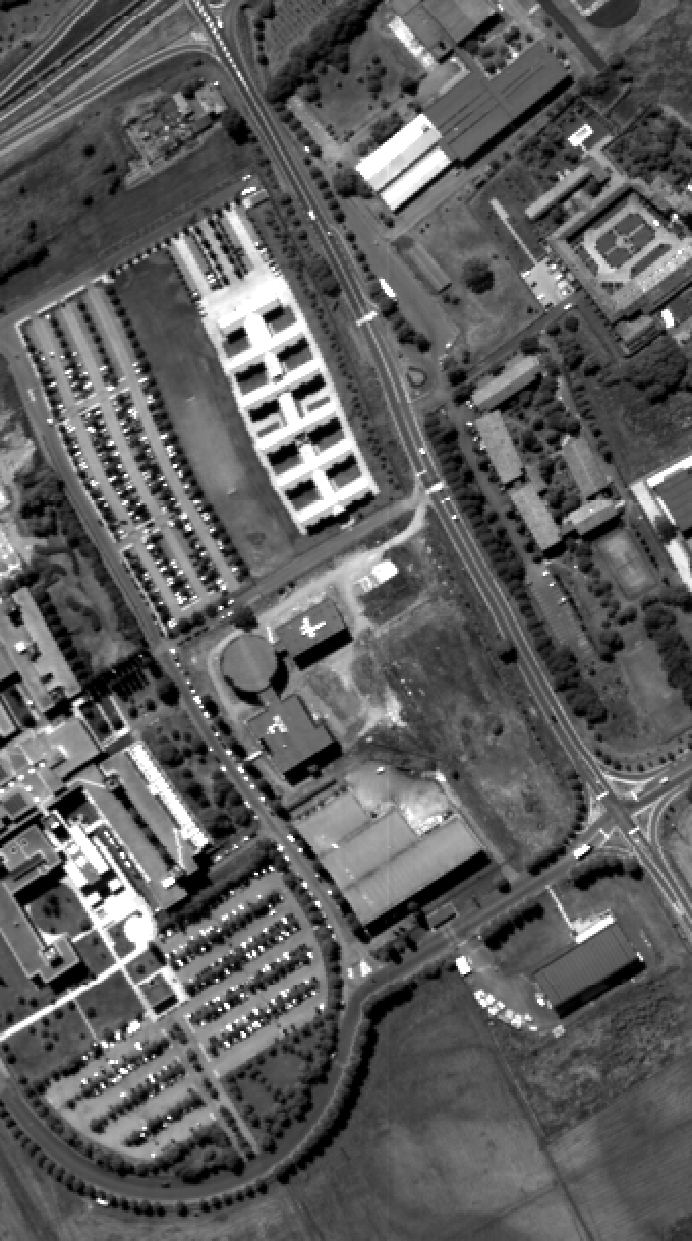
\includegraphics[trim=2.944cm 8.832cm 2.944cm 10.304cm, clip=true,width=0.22\linewidth]{./figures/university_pc1.png}
\end{center}

\begin{columns}
\begin{column}{0.22\columnwidth}
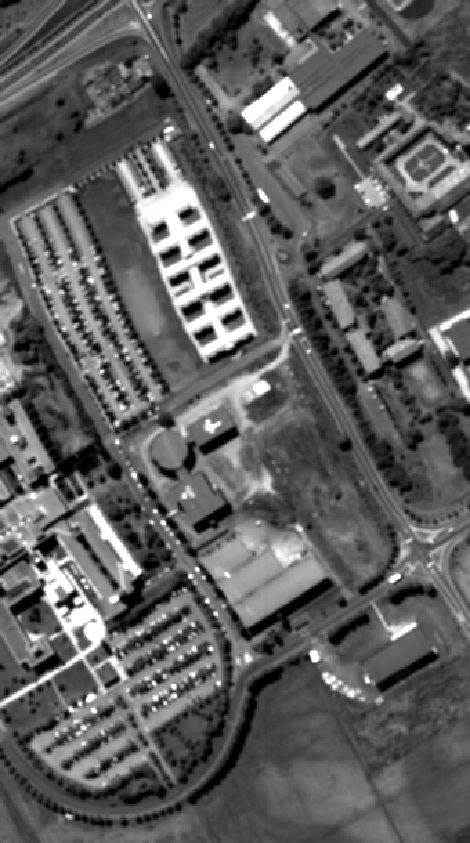
\includegraphics[trim=2cm 6cm 2cm 7cm, clip=true,width=1\linewidth]{./figures/university_pc1_mean_3_3.png}
\end{column}
\begin{column}{0.22\columnwidth}
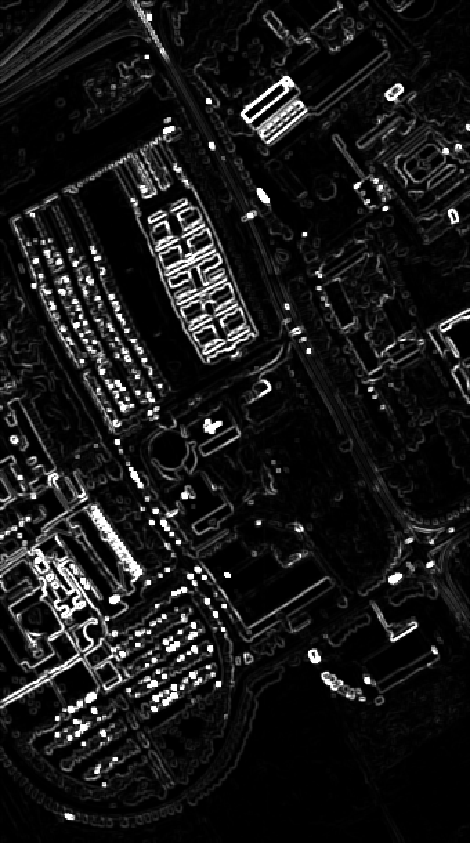
\includegraphics[trim=2cm 6cm 2cm 7cm, clip=true,width=1\linewidth]{./figures/university_pc1_std_3_3.png}
\end{column}
\begin{column}{0.22\columnwidth}
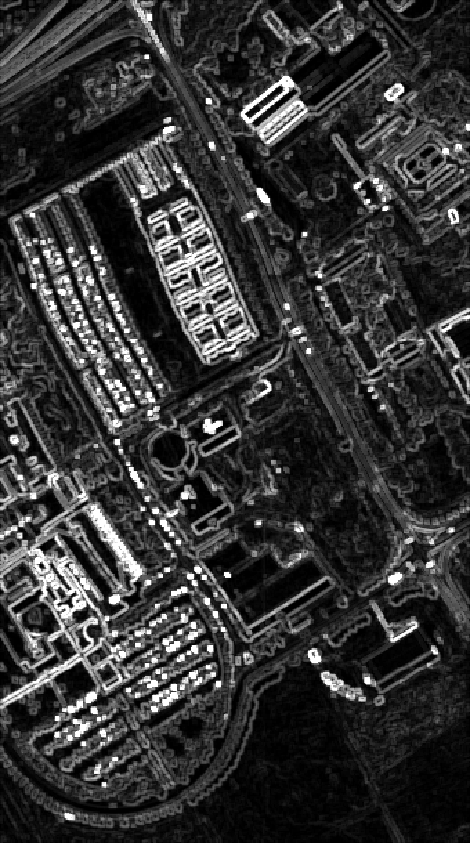
\includegraphics[trim=2cm 6cm 2cm 7cm, clip=true,width=1\linewidth]{./figures/university_pc1_range_3_3.png}
\end{column}
\begin{column}{0.22\columnwidth}
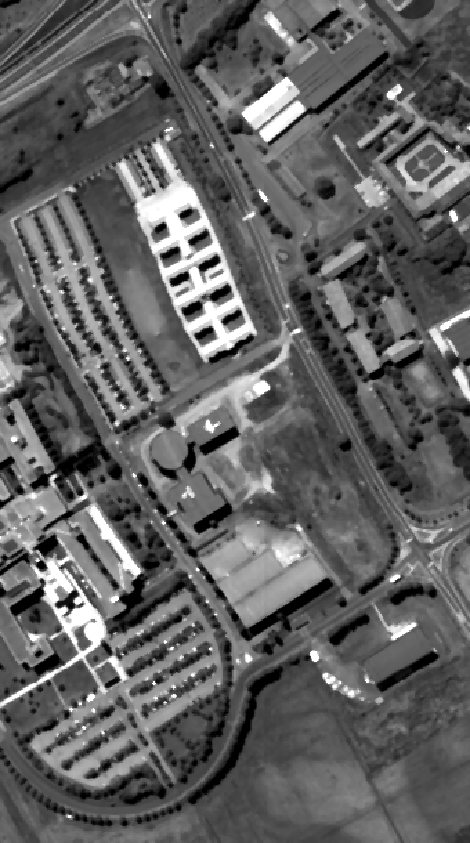
\includegraphics[trim=2cm 6cm 2cm 7cm, clip=true,width=1\linewidth]{./figures/university_pc1_median_3_3.png}
\end{column}
\end{columns}
\end{frame}
\begin{frame}[label={sec:orgc6786a5}]{Template filters in action 3/3}
\begin{center}
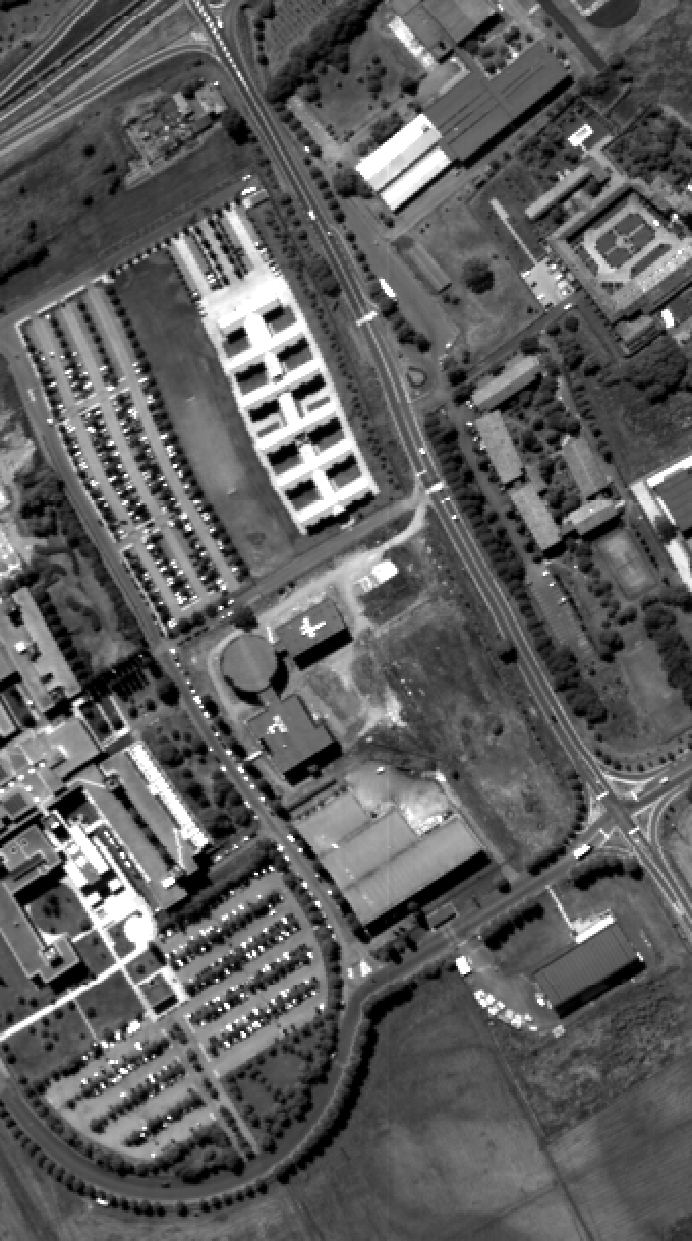
\includegraphics[trim=2.944cm 8.832cm 2.944cm 10.304cm, clip=true,width=0.22\linewidth]{./figures/university_pc1.png}
\end{center}

\begin{columns}
\begin{column}{0.22\columnwidth}
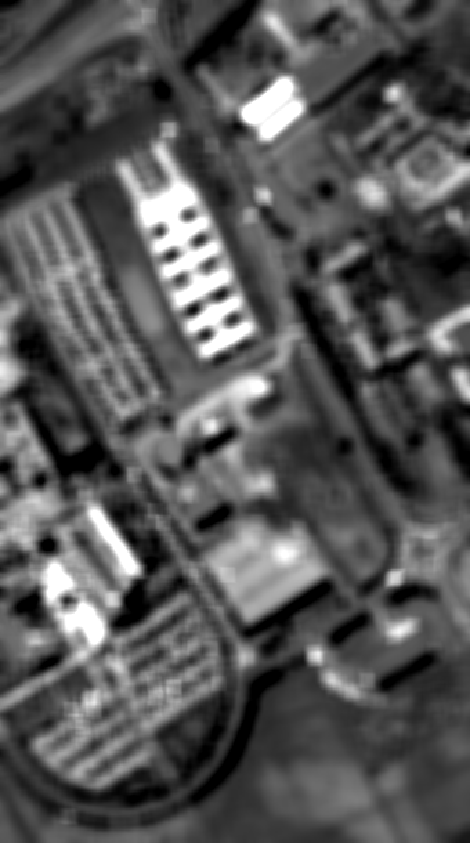
\includegraphics[trim=2cm 6cm 2cm 7cm, clip=true,width=1\linewidth]{./figures/university_pc1_mean_11_11.png}
\end{column}
\begin{column}{0.22\columnwidth}
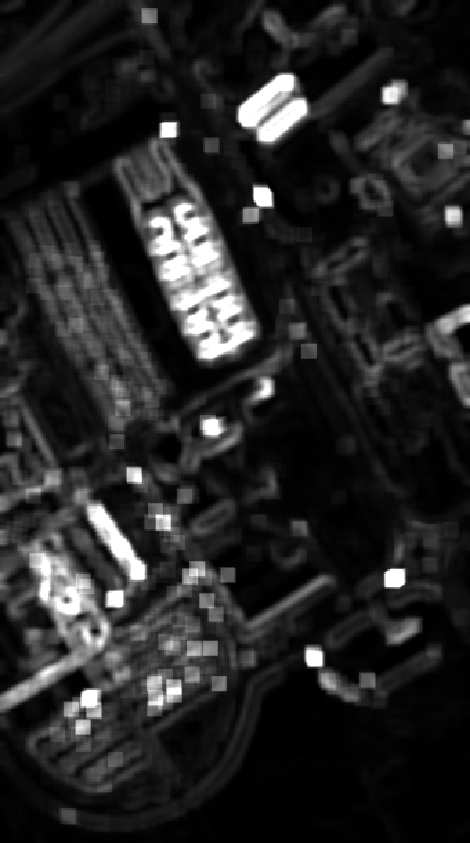
\includegraphics[trim=2cm 6cm 2cm 7cm, clip=true,width=1\linewidth]{./figures/university_pc1_std_11_11.png}
\end{column}
\begin{column}{0.22\columnwidth}
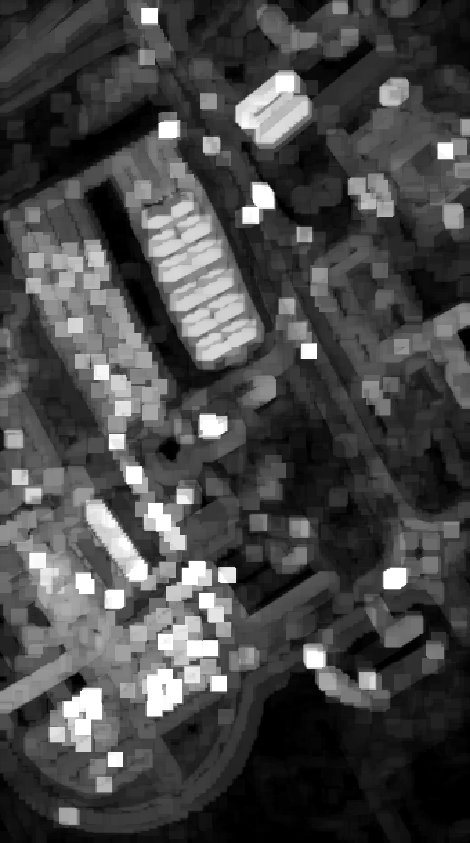
\includegraphics[trim=2cm 6cm 2cm 7cm, clip=true,width=1\linewidth]{./figures/university_pc1_range_11_11.png}
\end{column}
\begin{column}{0.22\columnwidth}
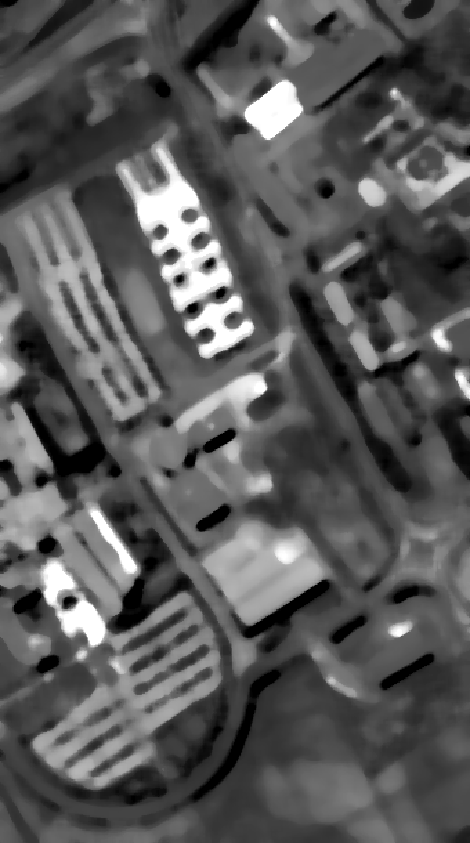
\includegraphics[trim=2cm 6cm 2cm 7cm, clip=true,width=1\linewidth]{./figures/university_pc1_median_11_11.png}
\end{column}
\end{columns}
\end{frame}
\subsection{Mathematical morphology}
\label{sec:orgbaae4e0}
\begin{frame}[label={sec:org0d9c061}]{Dilation and erosion}
\begin{itemize}
\item Mathematical morphology: non-linear image processing.
\item A lot of applications in geoscience and remote sensing, see \cite{soille:pesaresi}
\item \uline{Erosion}: template filter with a \(\min\) operation in \(G\) (called \emph{structuring element})
\item \uline{Dilation}: template filter with a \(\max\) operation in \(G\)
\end{itemize}

\begin{columns}
\begin{column}{0.3\columnwidth}
\begin{figure}[htbp]

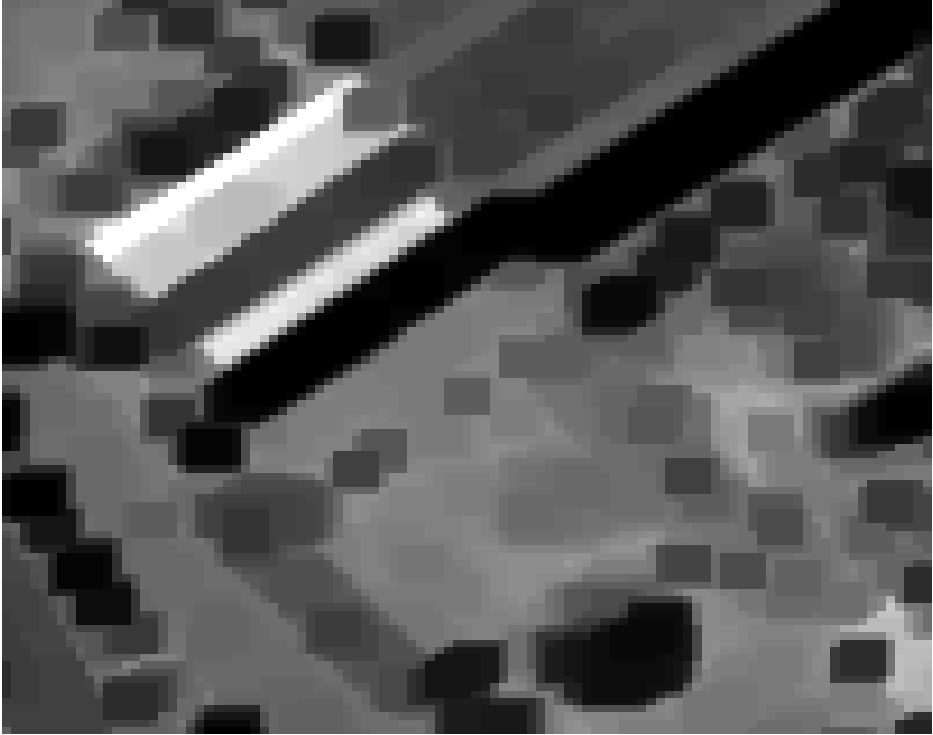
\includegraphics[width=0.85\linewidth,height=0.85\linewidth]{./figures/ero.pdf}
\end{figure}
\end{column}
\begin{column}{0.3\columnwidth}
\begin{figure}[htbp]

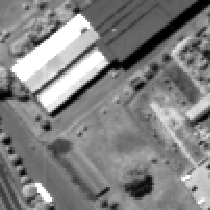
\includegraphics[width=0.85\linewidth,height=0.85\linewidth]{./figures/orig.pdf}
\end{figure}
\end{column}
\begin{column}{0.3\columnwidth}
\begin{figure}[htbp]

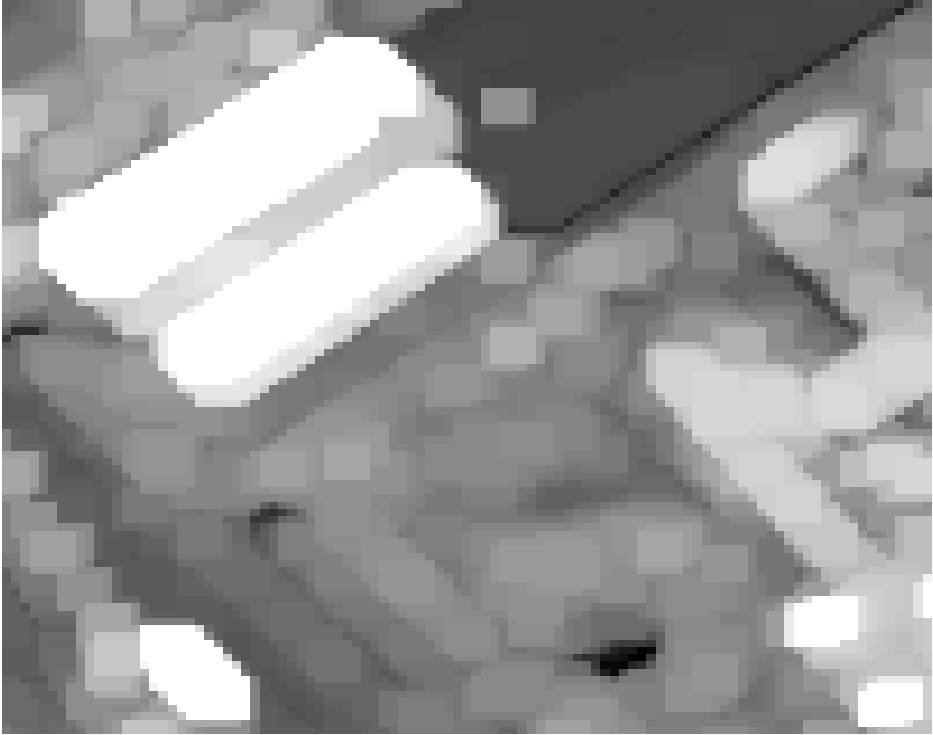
\includegraphics[width=0.85\linewidth,height=0.85\linewidth]{./figures/dil.pdf}
\end{figure}
\end{column}
\end{columns}
\end{frame}
\begin{frame}[label={sec:org75db5f3}]{Effets of structuring elements}
\begin{columns}
\begin{column}{0.3\columnwidth}
\begin{figure}[htbp]

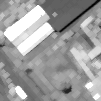
\includegraphics[width=0.85\linewidth,height=0.85\linewidth]{./figures/dil_disk.png}
\end{figure}

\begin{center}
\begin{tabular}{|c|c|c|c|c|}
\hline
0 & 0 & 1 & 0 & 0\\
\hline
0 & 1 & 1 & 1 & 0\\
\hline
1 & 1 & 1 & 1 & 1\\
\hline
0 & 1 & 1 & 1 & 0\\
\hline
0 & 0 & 1 & 0 & 0\\
\hline
\end{tabular}
\end{center}
\end{column}
\begin{column}{0.3\columnwidth}
\begin{figure}[htbp]

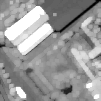
\includegraphics[width=0.85\linewidth,height=0.85\linewidth]{./figures/dil_square.png}
\end{figure}

\begin{center}
\begin{tabular}{|c|c|c|c|c|}
\hline
0 & 0 & 0 & 0 & 0\\
\hline
0 & 1 & 1 & 1 & 0\\
\hline
0 & 1 & 1 & 1 & 0\\
\hline
0 & 1 & 1 & 1 & 0\\
\hline
0 & 0 & 0 & 0 & 0\\
\hline
\end{tabular}
\end{center}
\end{column}

\begin{column}{0.3\columnwidth}
\begin{figure}[htbp]

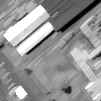
\includegraphics[width=0.85\linewidth,height=0.85\linewidth]{./figures/dil_line.png}
\end{figure}

\begin{center}
\begin{tabular}{|c|c|c|c|c|}
\hline
0 & 0 & 0 & 0 & 1\\
\hline
0 & 0 & 0 & 1 & 0\\
\hline
0 & 0 & 1 & 0 & 0\\
\hline
0 & 1 & 0 & 0 & 0\\
\hline
1 & 0 & 0 & 0 & 0\\
\hline
\end{tabular}
\end{center}
\end{column}
\end{columns}
\end{frame}

\begin{frame}[label={sec:orgf680d6f}]{Opening and closing}
\begin{itemize}
\item \uline{Opening}:
\begin{itemize}
\item \emph{Erosion} followed by a \emph{dilation}
\item Remove bright objects that are smaller than the SE
\end{itemize}
\item <2> \uline{Opening by reconstruction}:
\begin{itemize}
\item \emph{Erosion} followed by a \emph{reconstruction}
\item \emph{Completely} removes bright objects that are smaller than the SE, otherwise preserve it
\end{itemize}
\item \uline{Closing}:
\begin{itemize}
\item \emph{Dilation} followed by an \emph{erosion}
\item Remove dark objects that are smaller than the SE
\end{itemize}
\item <2> \uline{Closing by reconstruction}:
\begin{itemize}
\item \emph{Dilation} followed by an \emph{erosion}
\item \emph{Completely} removes dark objects that are smaller than the SE, otherwise preserve it
\end{itemize}
\end{itemize}

\begin{columns}
\begin{column}{0.2\columnwidth}
\begin{figure}[htbp]

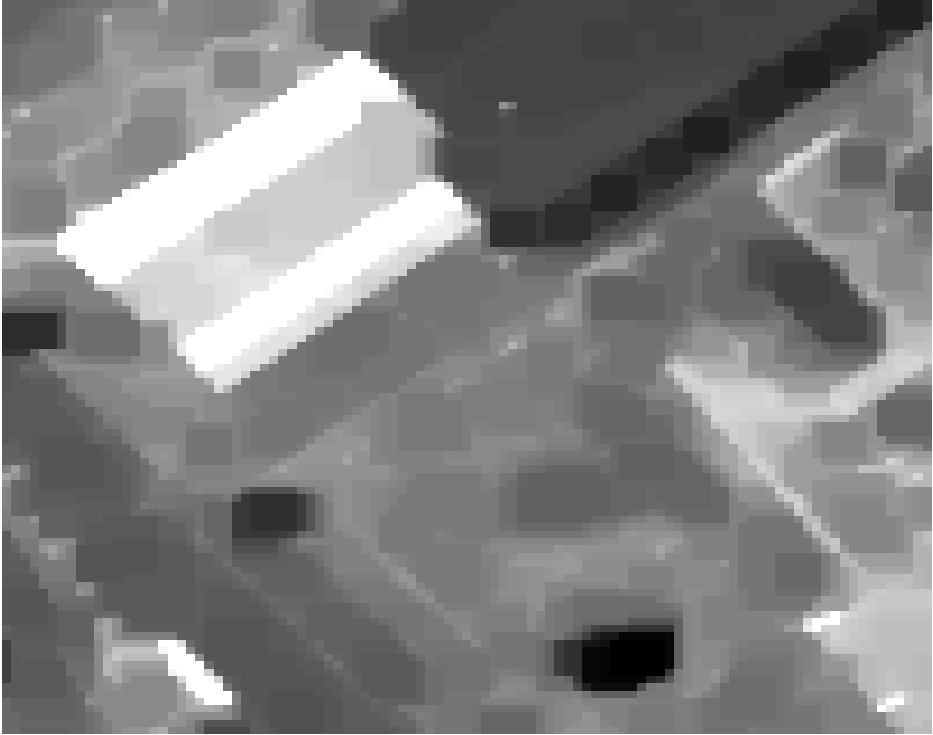
\includegraphics[width=1\linewidth,height=1\linewidth]{./figures/close.pdf}
\end{figure}
\end{column}
\begin{column}{0.2\columnwidth}
\only<2>{
\begin{figure}[htbp]

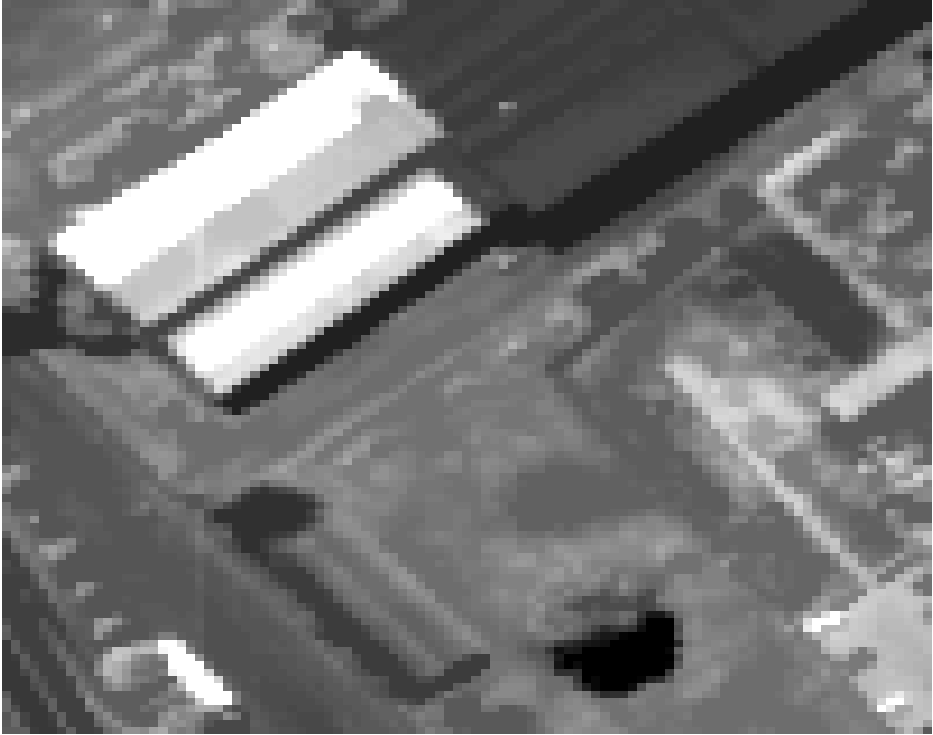
\includegraphics[width=1\linewidth,height=1\linewidth]{./figures/geo_close.pdf}
\end{figure}
}
\end{column}
\begin{column}{0.2\columnwidth}
\begin{figure}[htbp]

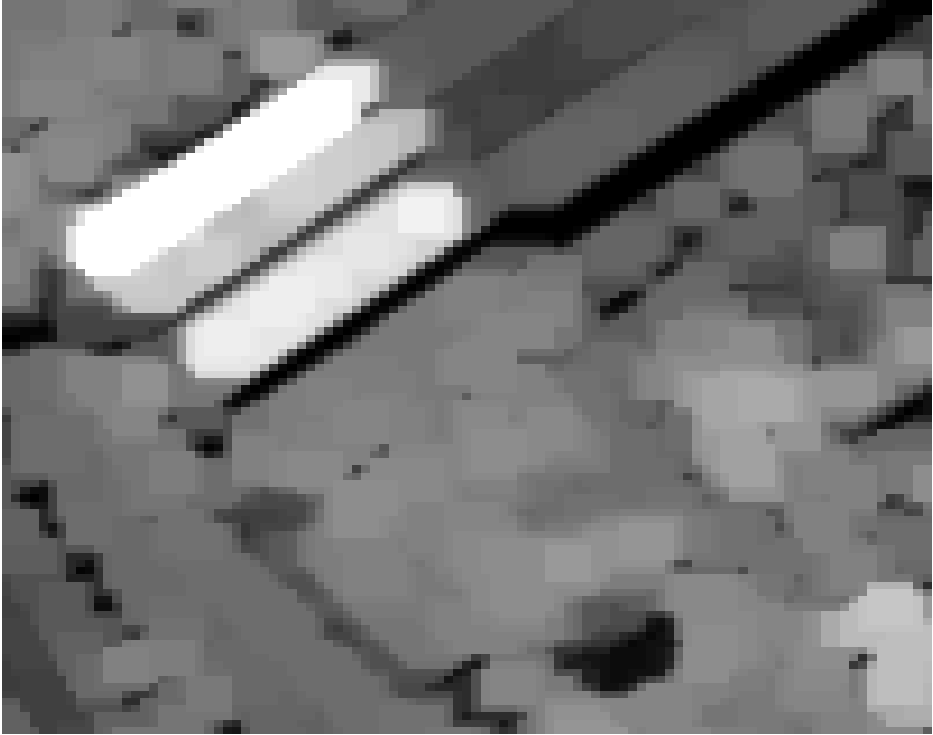
\includegraphics[width=1\linewidth,height=1\linewidth]{./figures/open.pdf}
\end{figure}
\end{column}
\begin{column}{0.2\columnwidth}
\only<2>{
\begin{figure}[htbp]

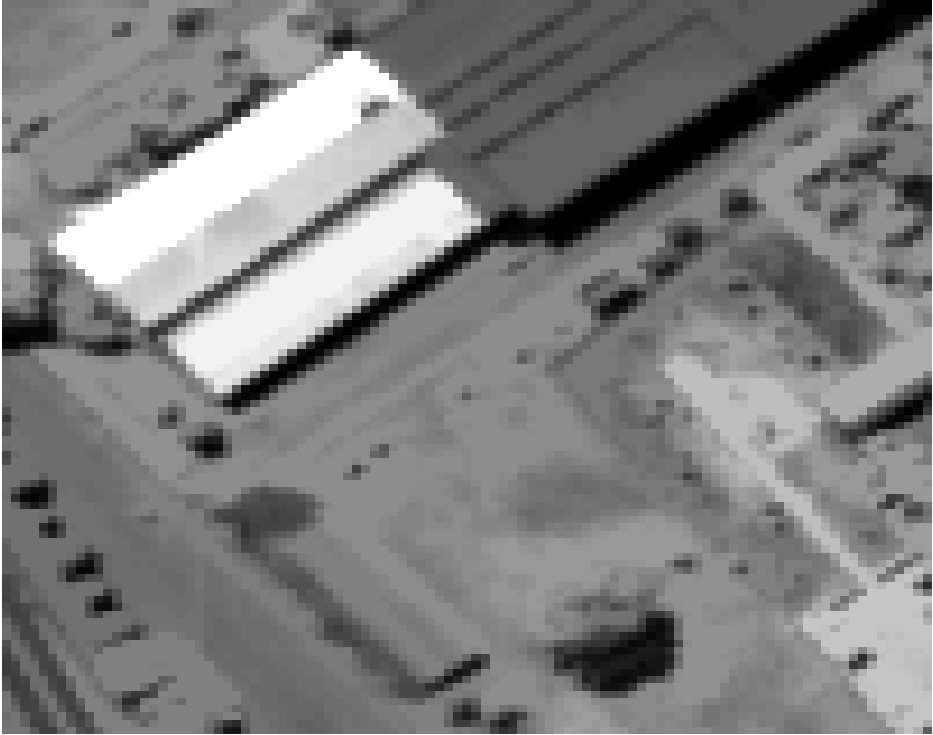
\includegraphics[width=1\linewidth,height=1\linewidth]{./figures/geo_open.pdf}
\end{figure}
}
\end{column}
\end{columns}
\end{frame}
\begin{frame}[label={sec:org7df92e2}]{Opening and closing profile}
\begin{itemize}
\item For a  given \(B\),  \(\gamma_{B}^r\)  (resp. \(\phi_{B}^r\))   indicates which clear (dark) objects fit \(B\).
\begin{center}
  \begin{tikzpicture}[]
    \node at (0,0) {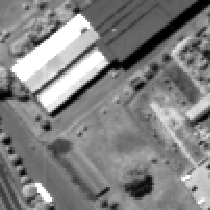
\includegraphics[width=0.2\textwidth,height=0.215\textheight]{figures/orig}};
    \node at (5,0) {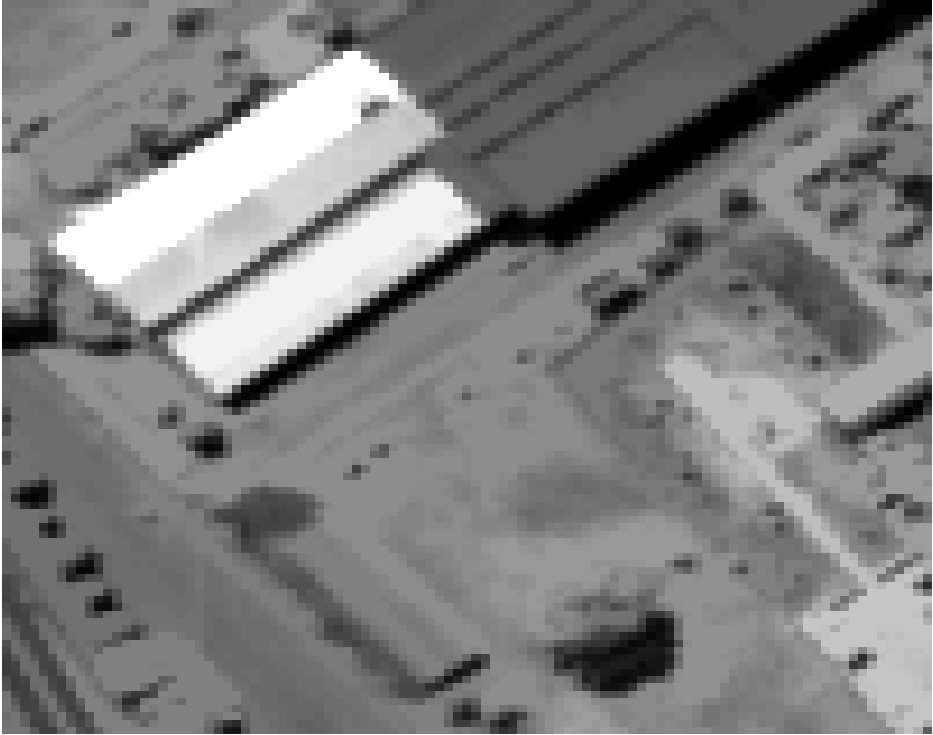
\includegraphics[width=0.2\textwidth,height=0.215\textheight]{figures/geo_open}};
    \node at (10,0) {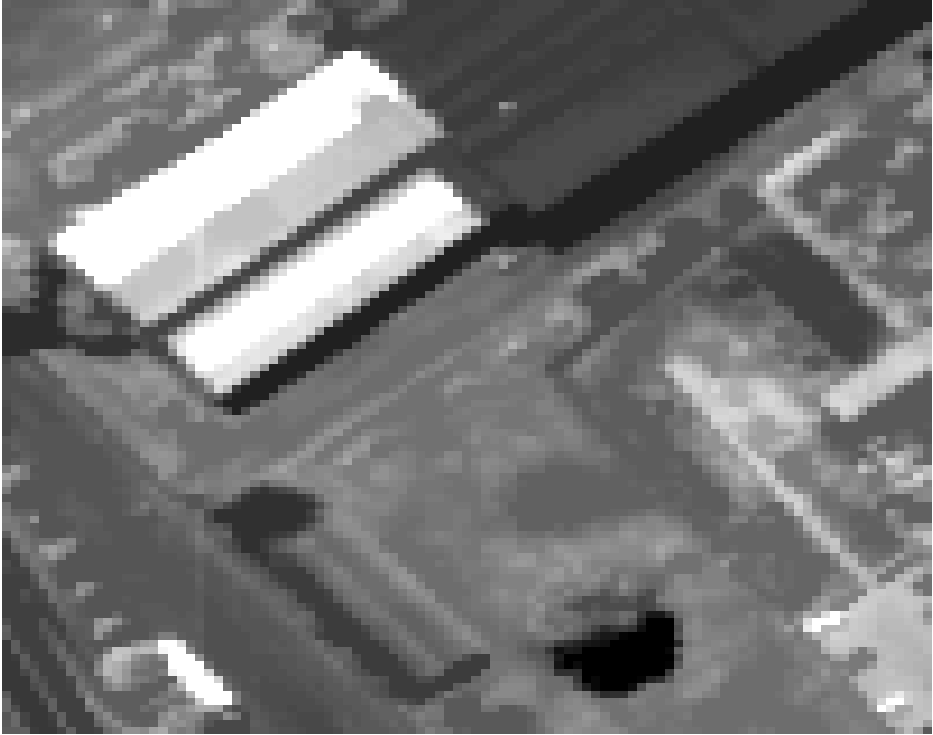
\includegraphics[width=0.2\textwidth,height=0.215\textheight]{figures/geo_close}};
    \draw[->,red,very thick] (-0.9,-0.85) -- node[above] {$\gamma_{B}^r$} (4,-0.85);
    \draw[->,red,very thick] (-0.85,-0.15) -- node[above] {$\phi_{B}^r$} (9,-0.15);
  \end{tikzpicture}
\end{center}
\item Applying \(\gamma_{B_i}\) with a set of \(\big\{B_i|B_{i}\subset B_{i+1},i\in[1,\ldots,n]\big\}\) : \textcolor{magenta}{Opening Profile}
\item Applying \(\phi_{B_i}\) with a set of \(\big\{B_i|B_{i}\subset B_{i+1},i\in[1,\ldots,n]\big\}\) : \textcolor{magenta}{Closing Profile}
\end{itemize}
\end{frame}
\subsection{Extension to multivalued images}
\label{sec:org1b2ae1b}
\begin{frame}[label={sec:orgb5b1257}]{Ordering relation}
\begin{itemize}
\item MM is based on \(\inf\) and \(\sup\) operators
\item No unambiguous \$\(\inf\)\$/\(\sup\) for pixel/vector:
$$\begin{bmatrix}1\\5\\2\end{bmatrix} \overset{?}{\lessgtr} \begin{bmatrix}0\\6\\1\end{bmatrix}$$
\item Marginal ordering \(\Rightarrow\) by band filtering
\item Reduced ordering \(\Rightarrow h:\mathbb{R}^d\to\mathbb{R}\)
$$\mathbf{x}\mapsto h(x)$$
\item Use spectral feature extractio \emph{then} spatial feature extraction.
\end{itemize}
\end{frame}
\end{document}